\section{PRECIPITATIONS}


IN general, the forecast of precipitations is more complicated than temperature, thus the scores are a little less good for this part especially the deterministic ones. 



\subsection{Deterministic Evaluation Metrics}

\subsubsection{Spearman rank correlation}

\begin{figure}[H]
	\centering
	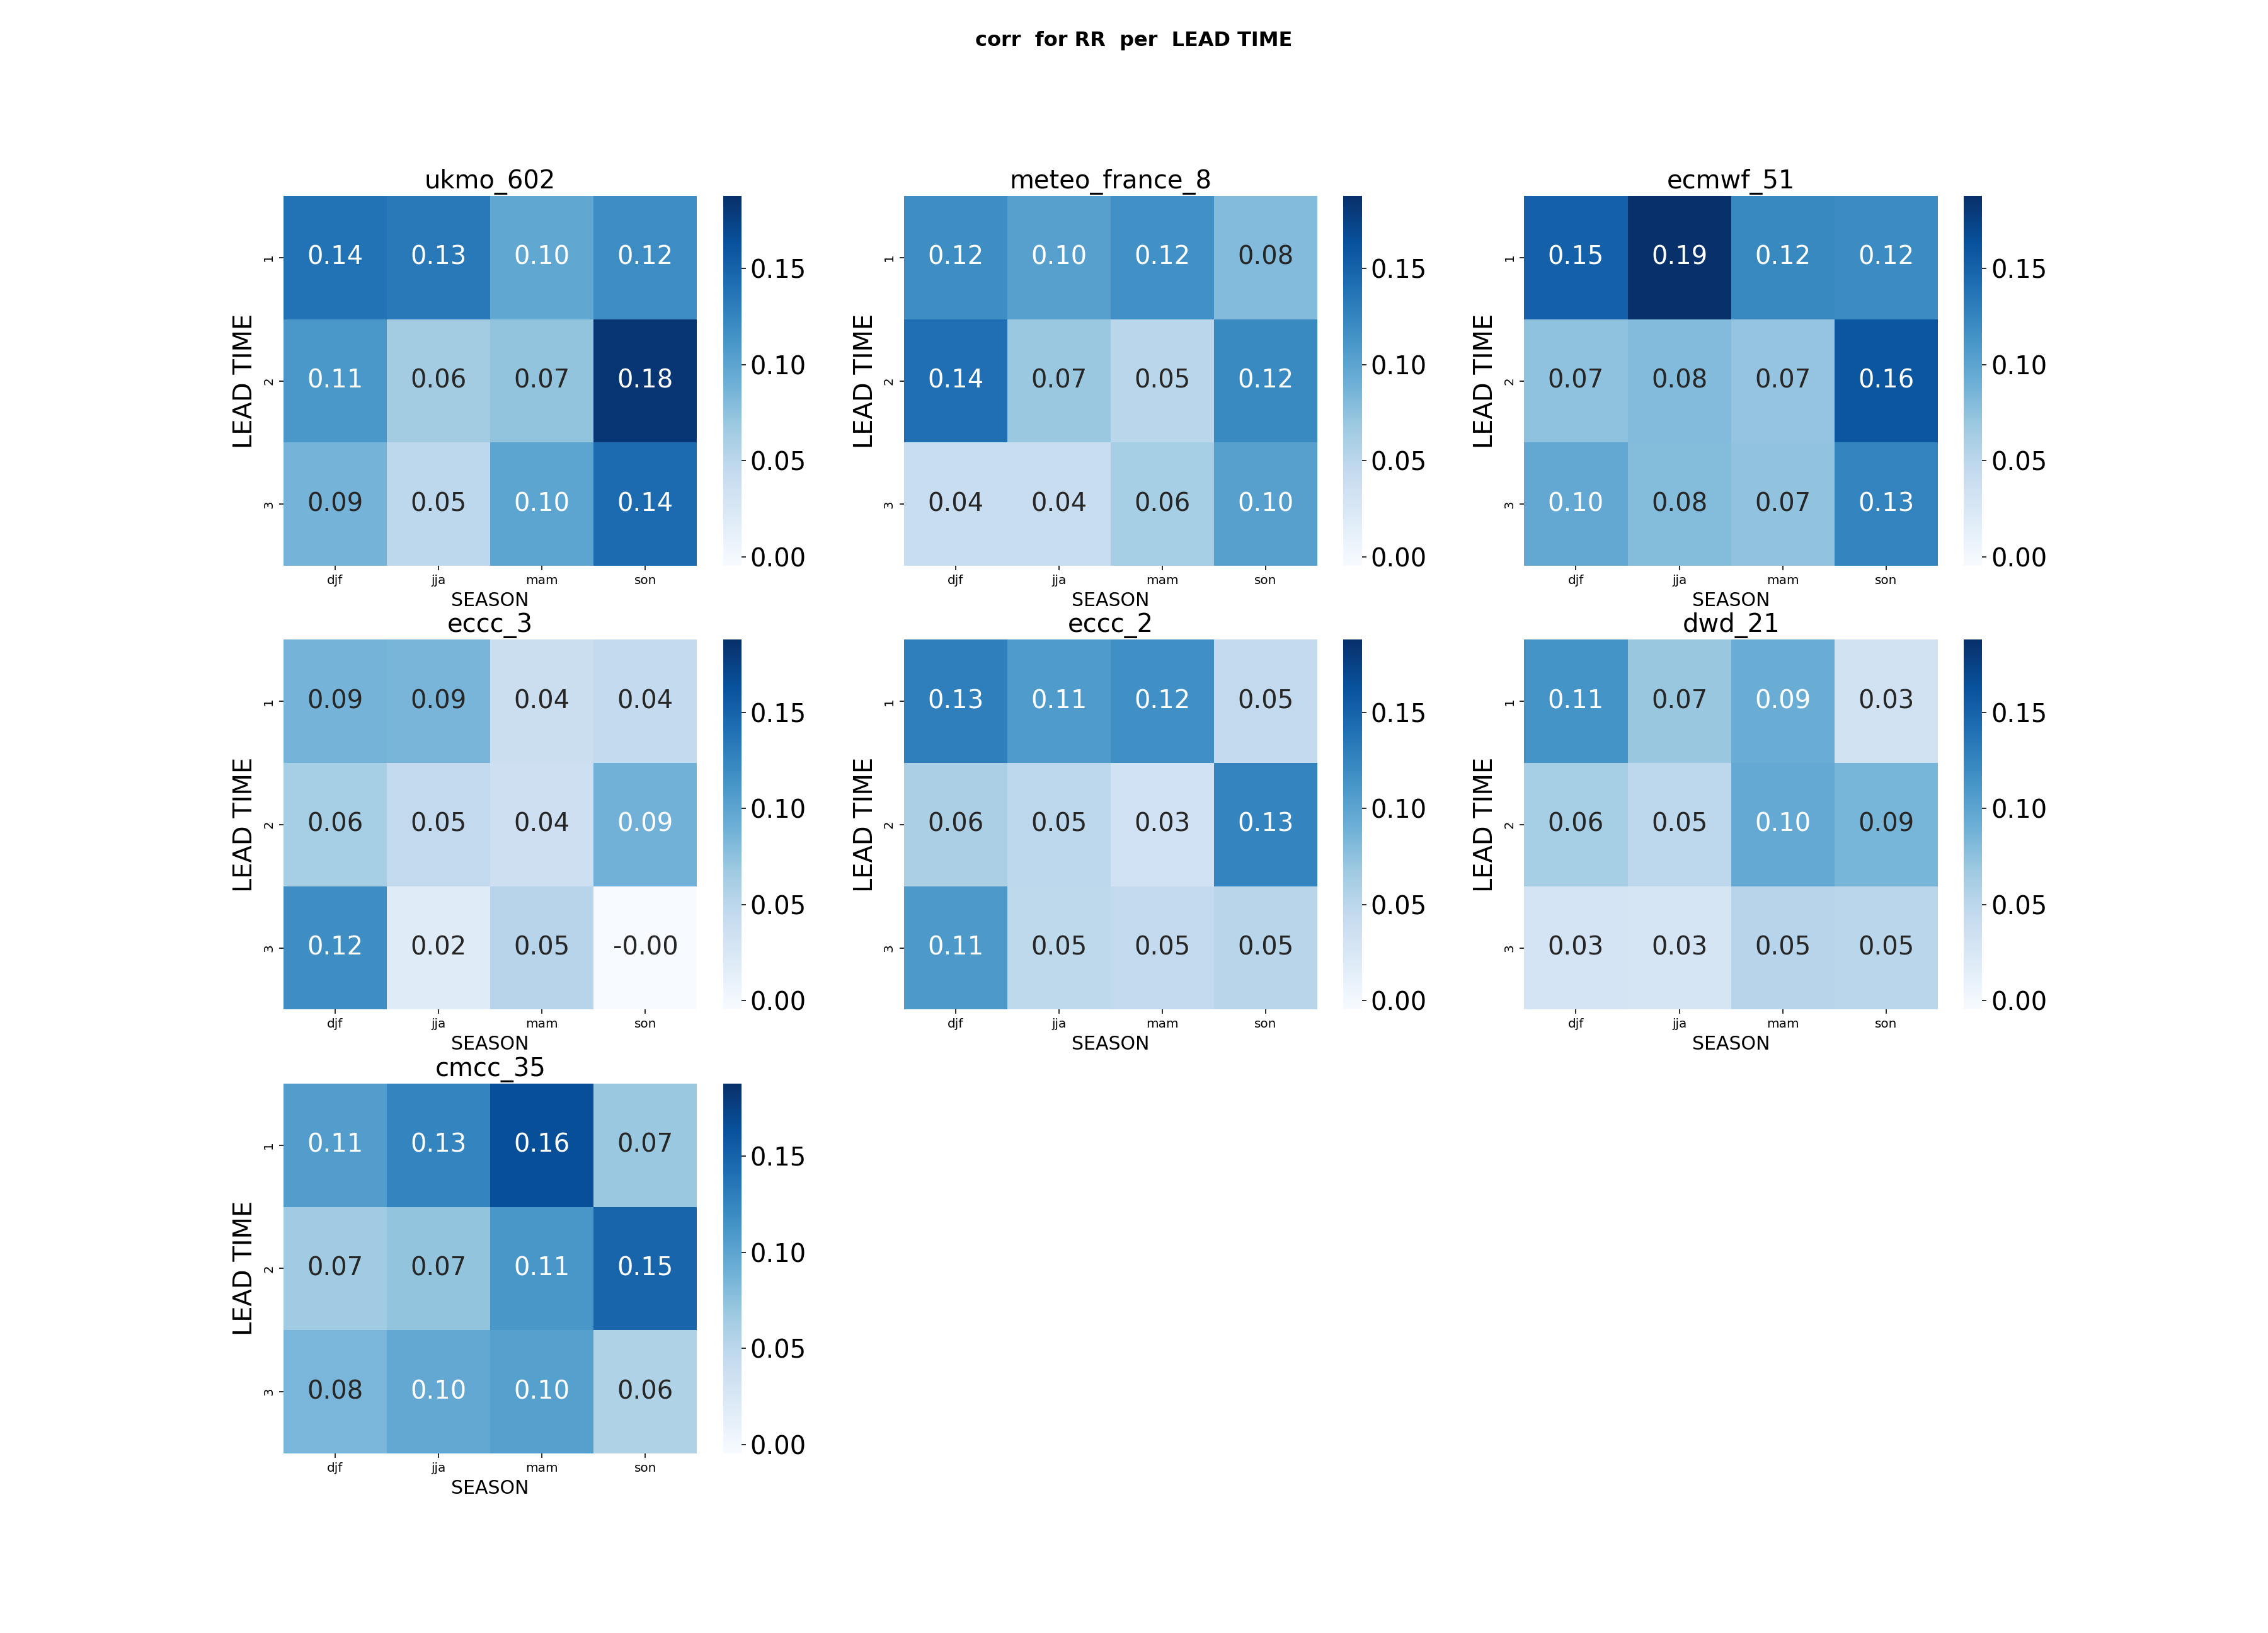
\includegraphics[scale=0.25]{plots/det/corr/corr_RR.png}
	\caption{The Heatmap of correlation for the mena region for every period \textbf{\textit{(1 for perfect Correlation)} }}
\end{figure}
The correlation is weak for all centers; however, the best models are \textbf{\textit{ECMWF, UKMO, and CMCC-35}}. There is no clear variability in performance along lead-time. For SON, the performance is excellent at lead-time 2 for all centers. As for the other seasons, the performance is generally strong at the 1st lead-time but decreases with increasing lead-time.
Hence, Meteo-France also shows good performance, but it decreases significantly over time.





\begin{figure}[H]
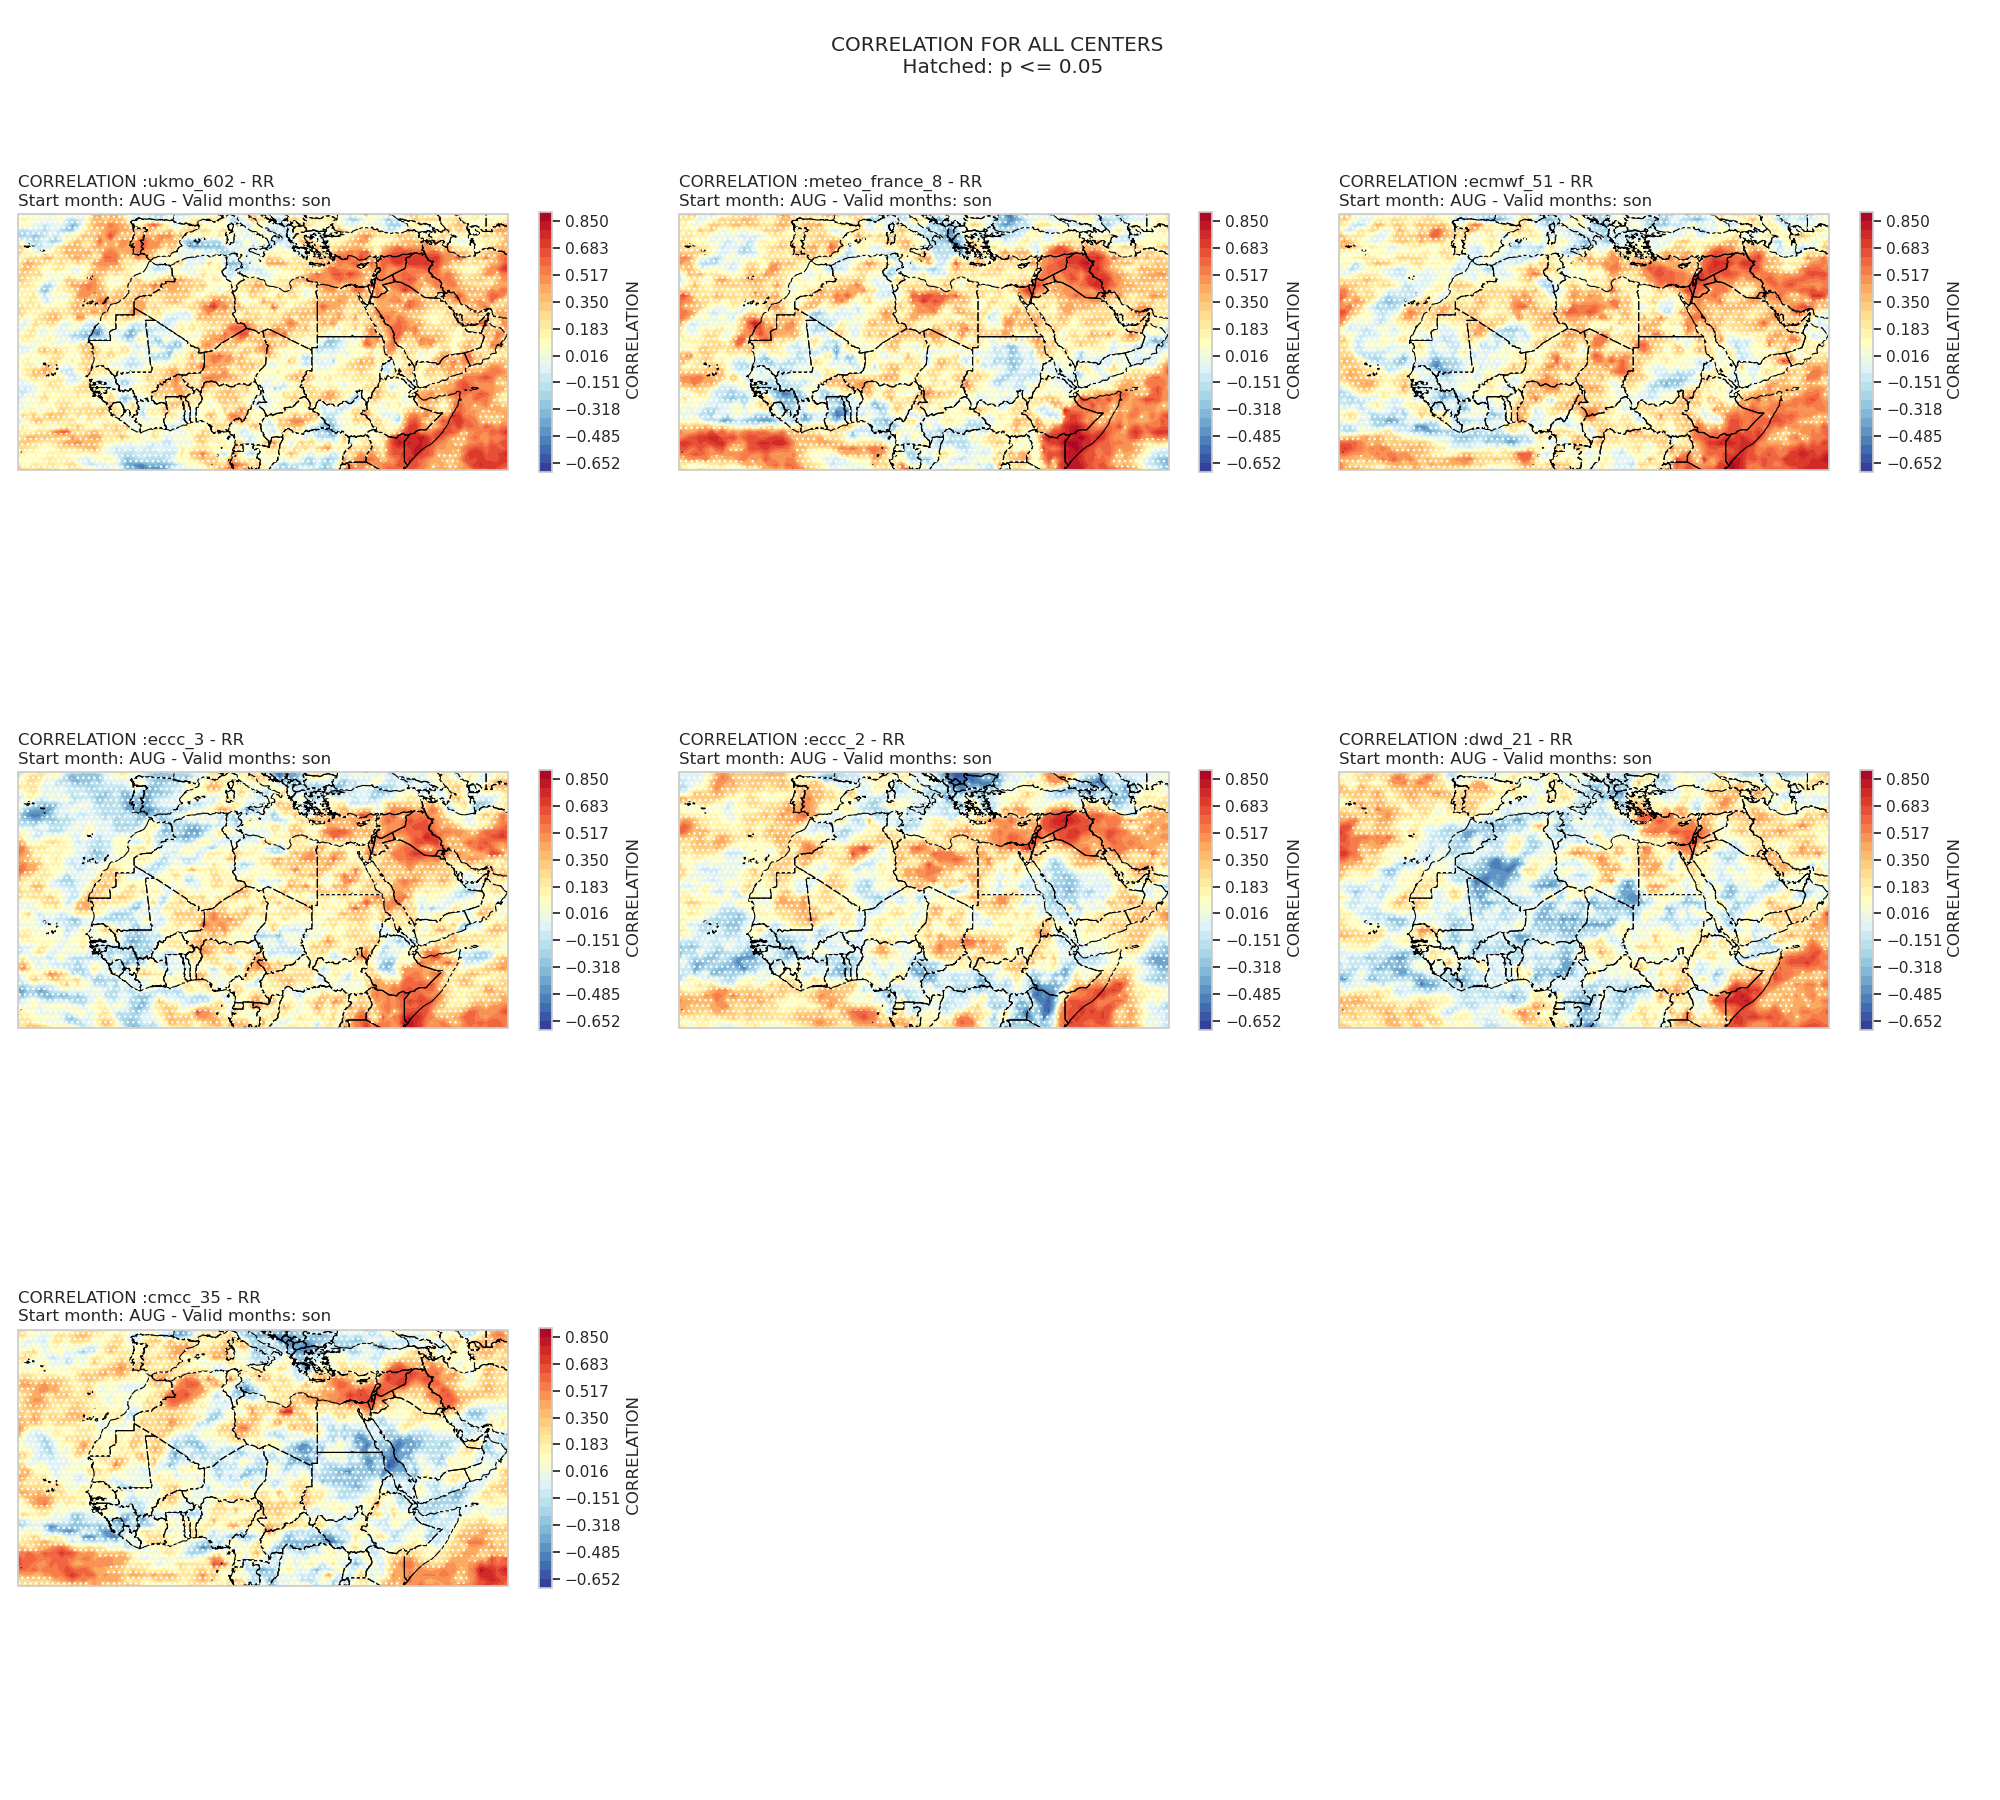
\includegraphics[scale=0.3]{plots/det/corr/CORR_son_RR.png}
\caption{3-months Rolling mean of Spearman Correlation in MENA Region for all centers SON}
\end{figure}
For temperature, the models demonstrate the best performance in the tropical regions. However, for precipitation, the situation is different. Hence the results show good performance during SON, where the Middle East, East Africa, and North Africa exhibit the highest correlation performance.
\begin{figure}[H]
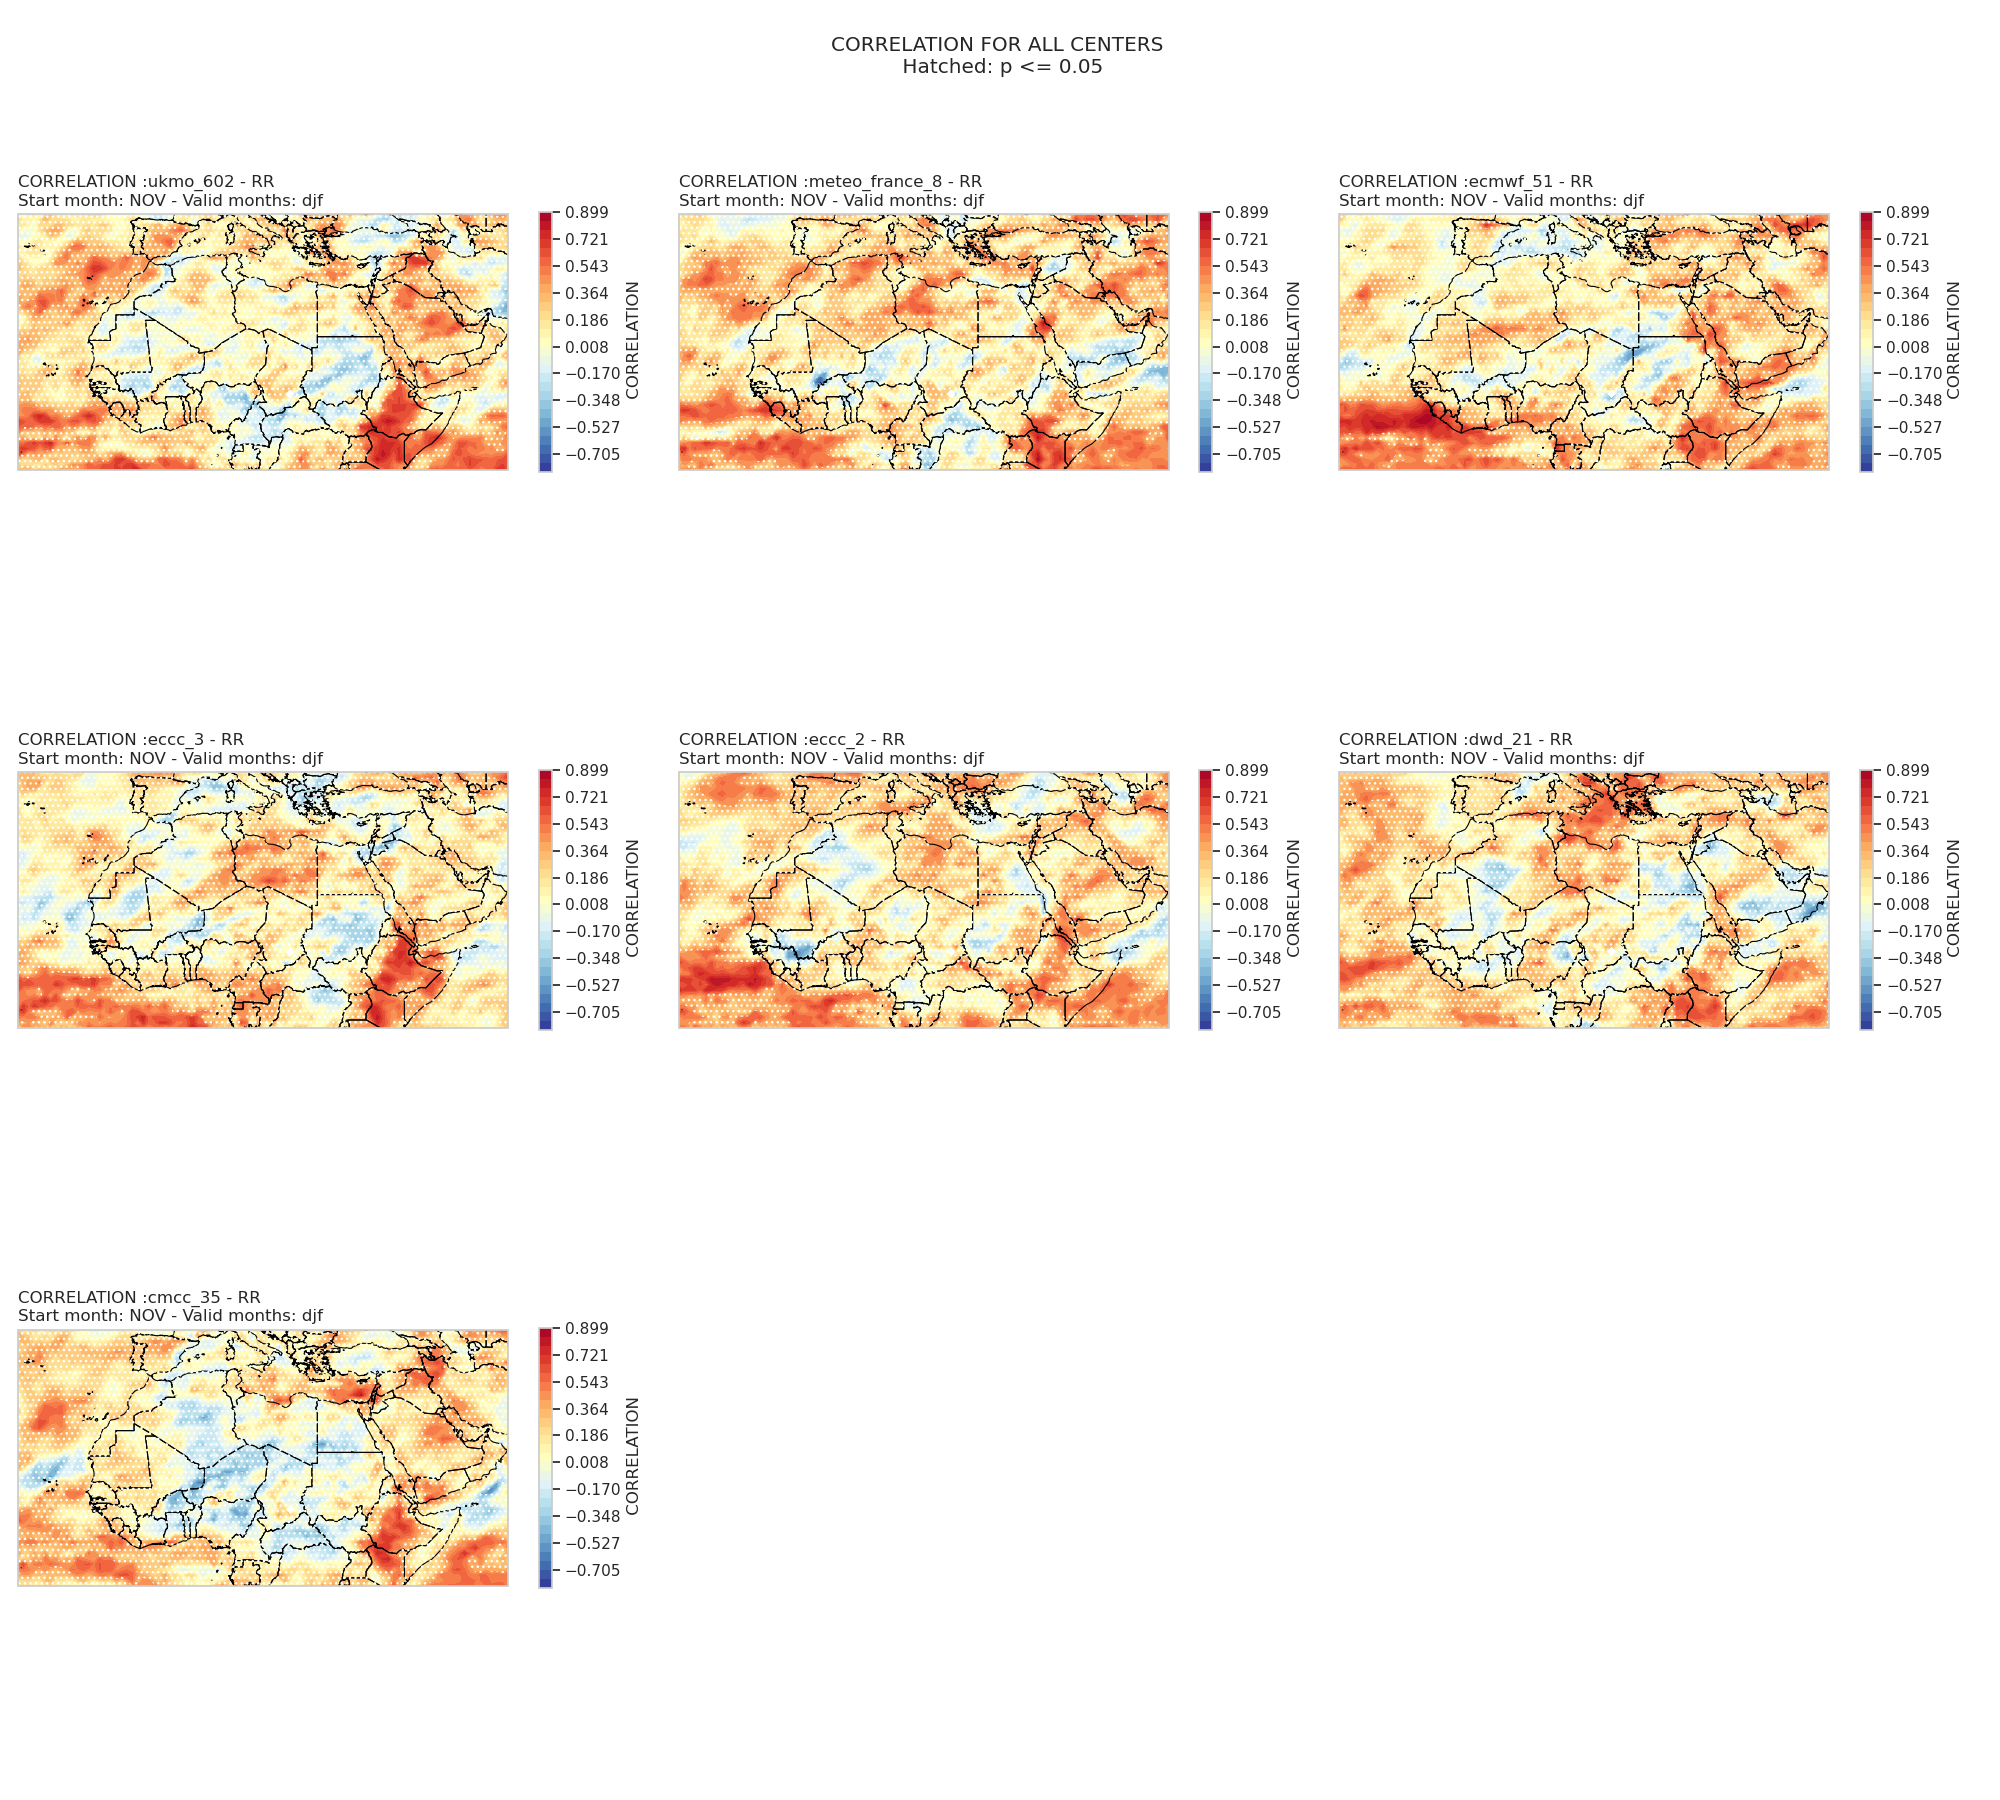
\includegraphics[scale=0.3]{plots/det/corr/CORR_djf_RR.png}
\caption{3-months Rolling mean of Spearman Correlation in MENA Region for all centers DJF}
\end{figure}

The 3-month rolling mean for SON correlation shows that the best models are \textbf{\textit{ECMWF, UKMO, and Meteo-France}}. The correlation is significant across most of the MENA region, except in the east of Africa, Palestine, Syria, Jordan, and Iraq, where the correlation is maximal, for all centers the Middle East and East of Africa are have the highest score. However, near the equator, the correlation is negative and weak. This results are confirmed in all centers.
 
For DJF, the situation is generally better than for SON. The best model for North Africa is \textbf{\textit{Meteo-France}}, as it shows good and significant correlation. In general, \textbf{\textit{ECMWF and Meteo-France}} are the best. In general we notice that there is differences between centers, especially in the Middle East and Center Africa.




\subsubsection{RMSE}
 
for the Root Mean Squared Error, the best models shown in the heatmap below are \textbf{\textit{DWD, ECMWF and UKMO}}. The RMSE score demonstrate an excellent performance for all models especially \textbf{\textit{DWD, ECMWF and UKMO}}. The performance is stable over lead-times and it is much better for djf in all centers.

\begin{figure}[H]
\includegraphics[scale=0.3]{plots/det/rmse/rmse_RR.png}
\caption{3-months Rolling mean of RMSE in MENA Region for all centers DJF}
\end{figure}

\begin{figure}[H]
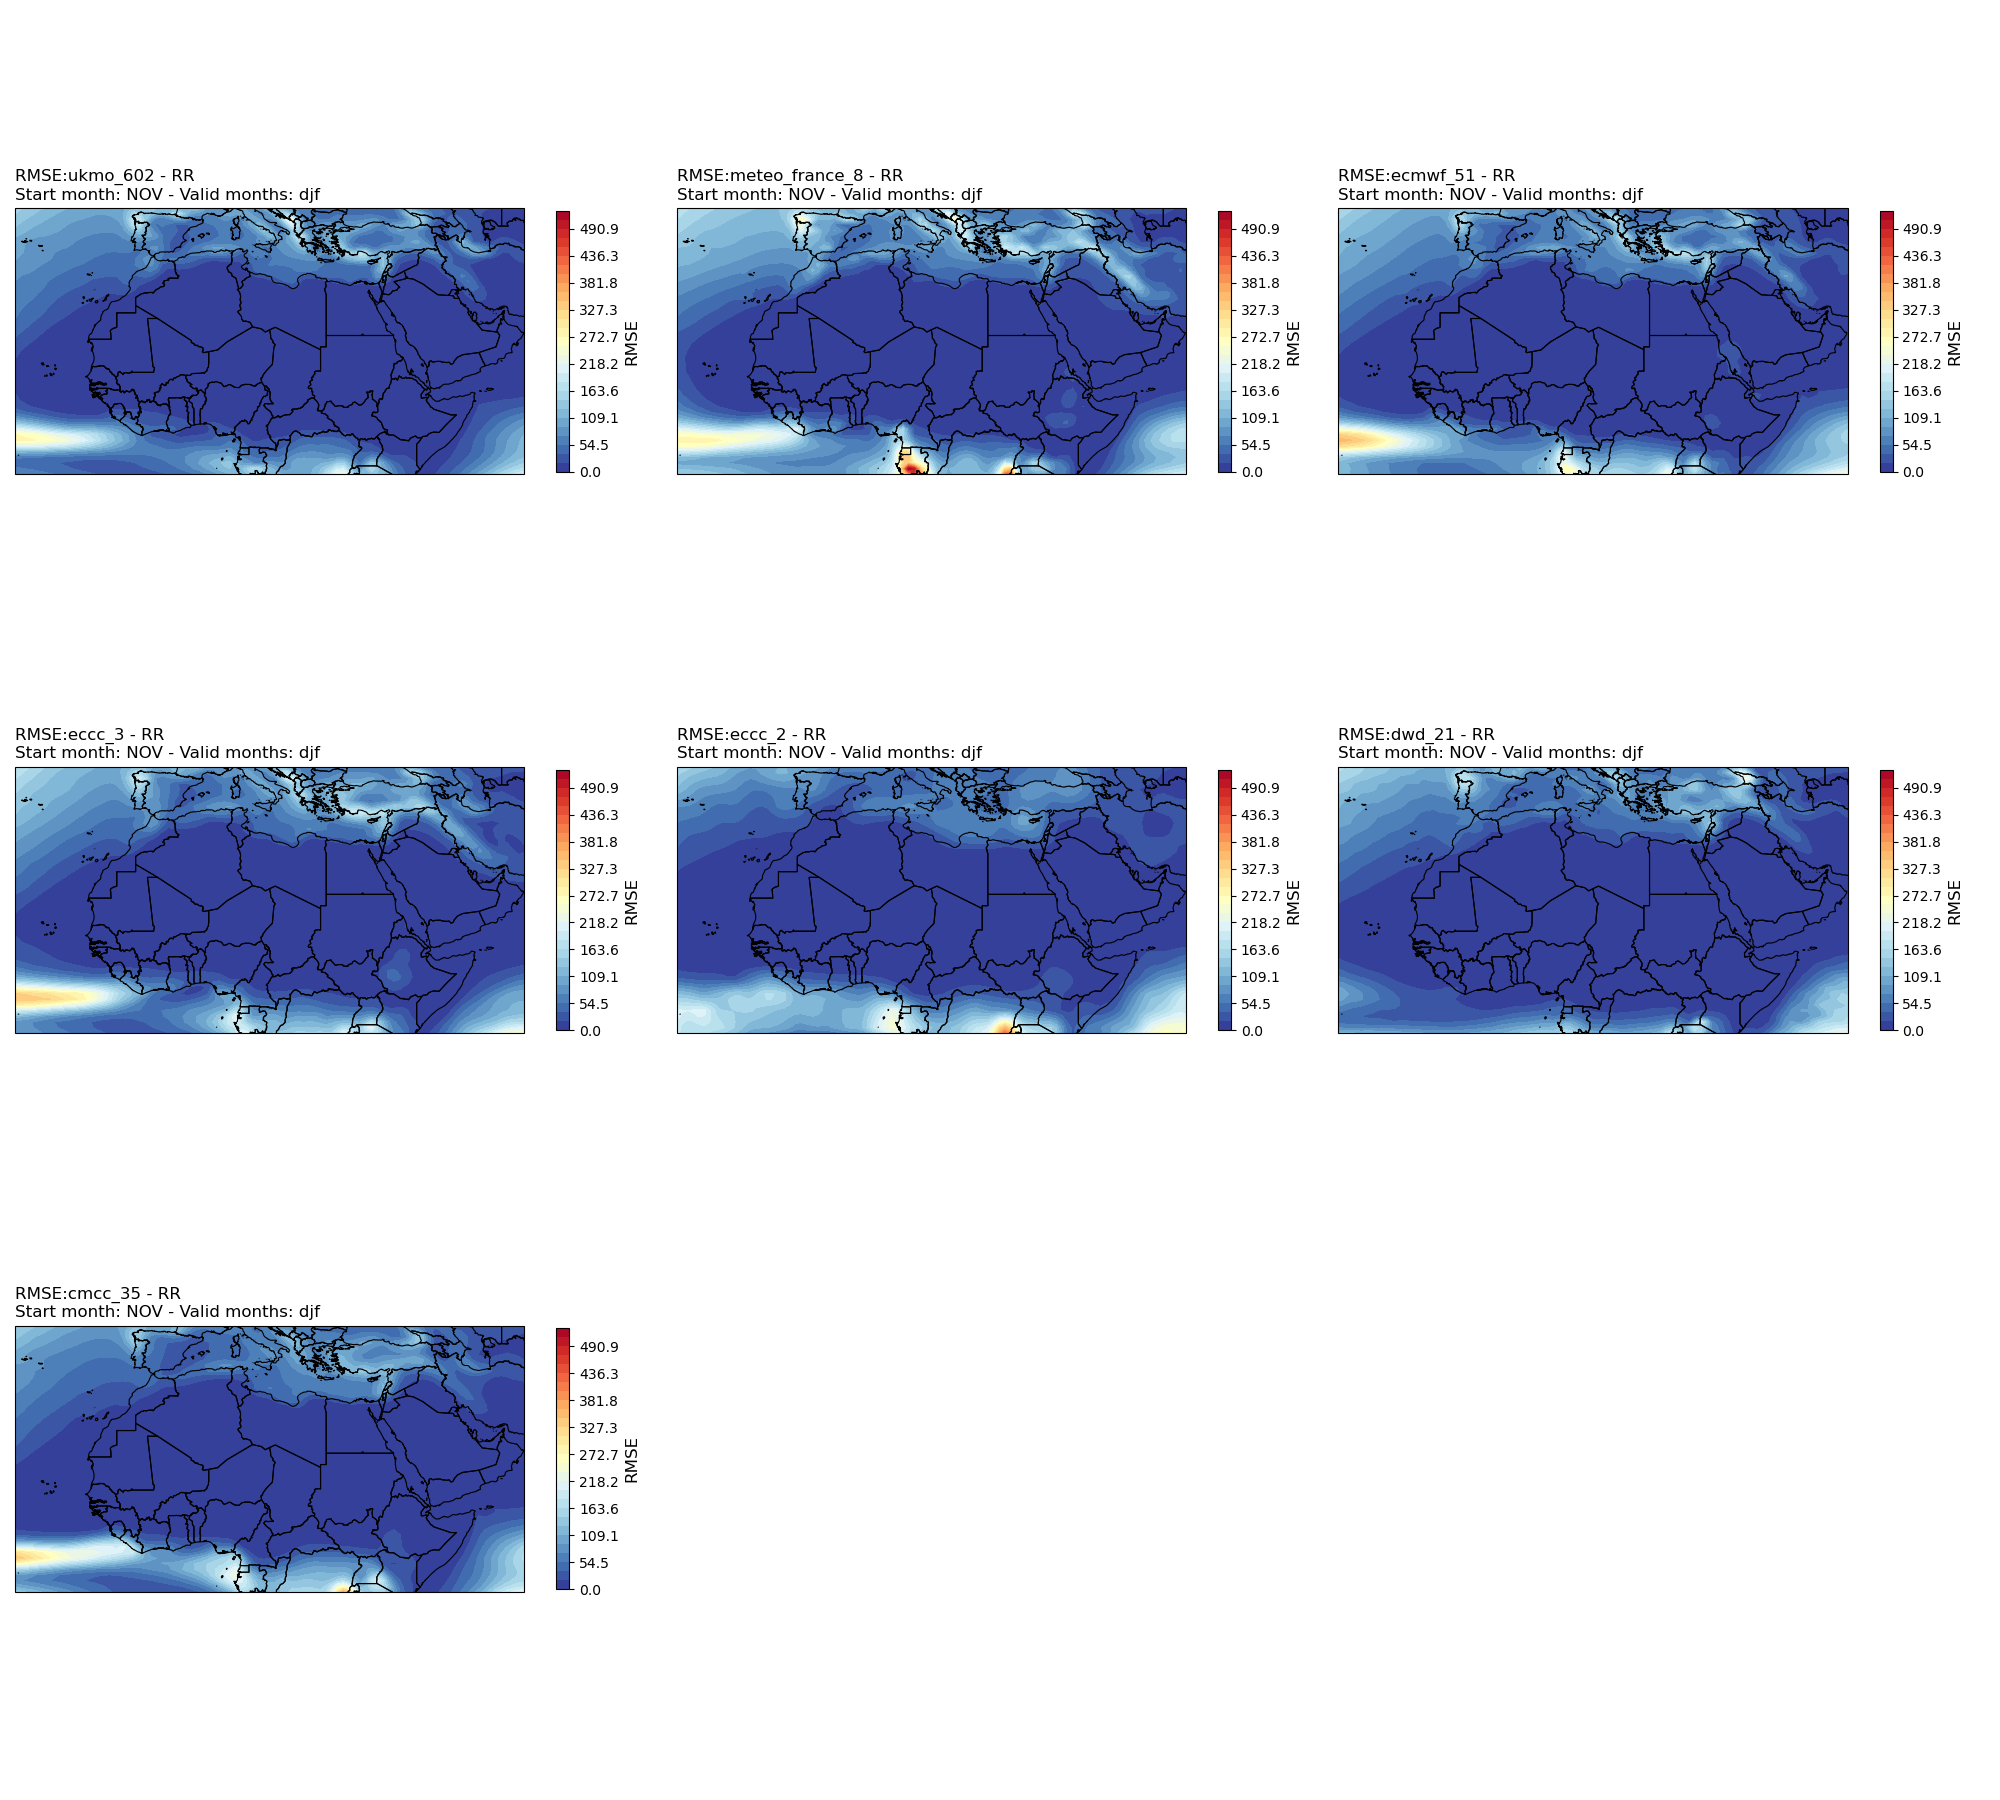
\includegraphics[scale=0.3]{plots/det/rmse/rmse_djf_RR.png}
\caption{3-months Rolling mean of RMSE in MENA Region for all centers JJA}
\end{figure}

also for the spacial dimension, the RMSE stay stable and exhibit very good performance for all centers. Thus, all models have high skill and they are consistent with each other.


\subsubsection{Coefficient of Determination (\( R^2 \))}
for precipitation, the R-SQUARED is very low, the maximum value is less than 0.1. However, the ecmwf is the best in term of R-SQUARED. for DJF,JJA and MAM the highest performance is in the first Lead-time, and it decrease along time, But for SON the best score is in the second Lead-time for all centers.
\begin{figure}[H]
	\centering
	\includegraphics[scale=0.25]{plots/det/rsquared/rsquared_RR.png}
	\caption{The Heatmap of rsquared for Precipitations in the mena region for every period \textbf{\textit{(1 for perfect RSQUARED)} }}
\end{figure}



\begin{figure}[H]
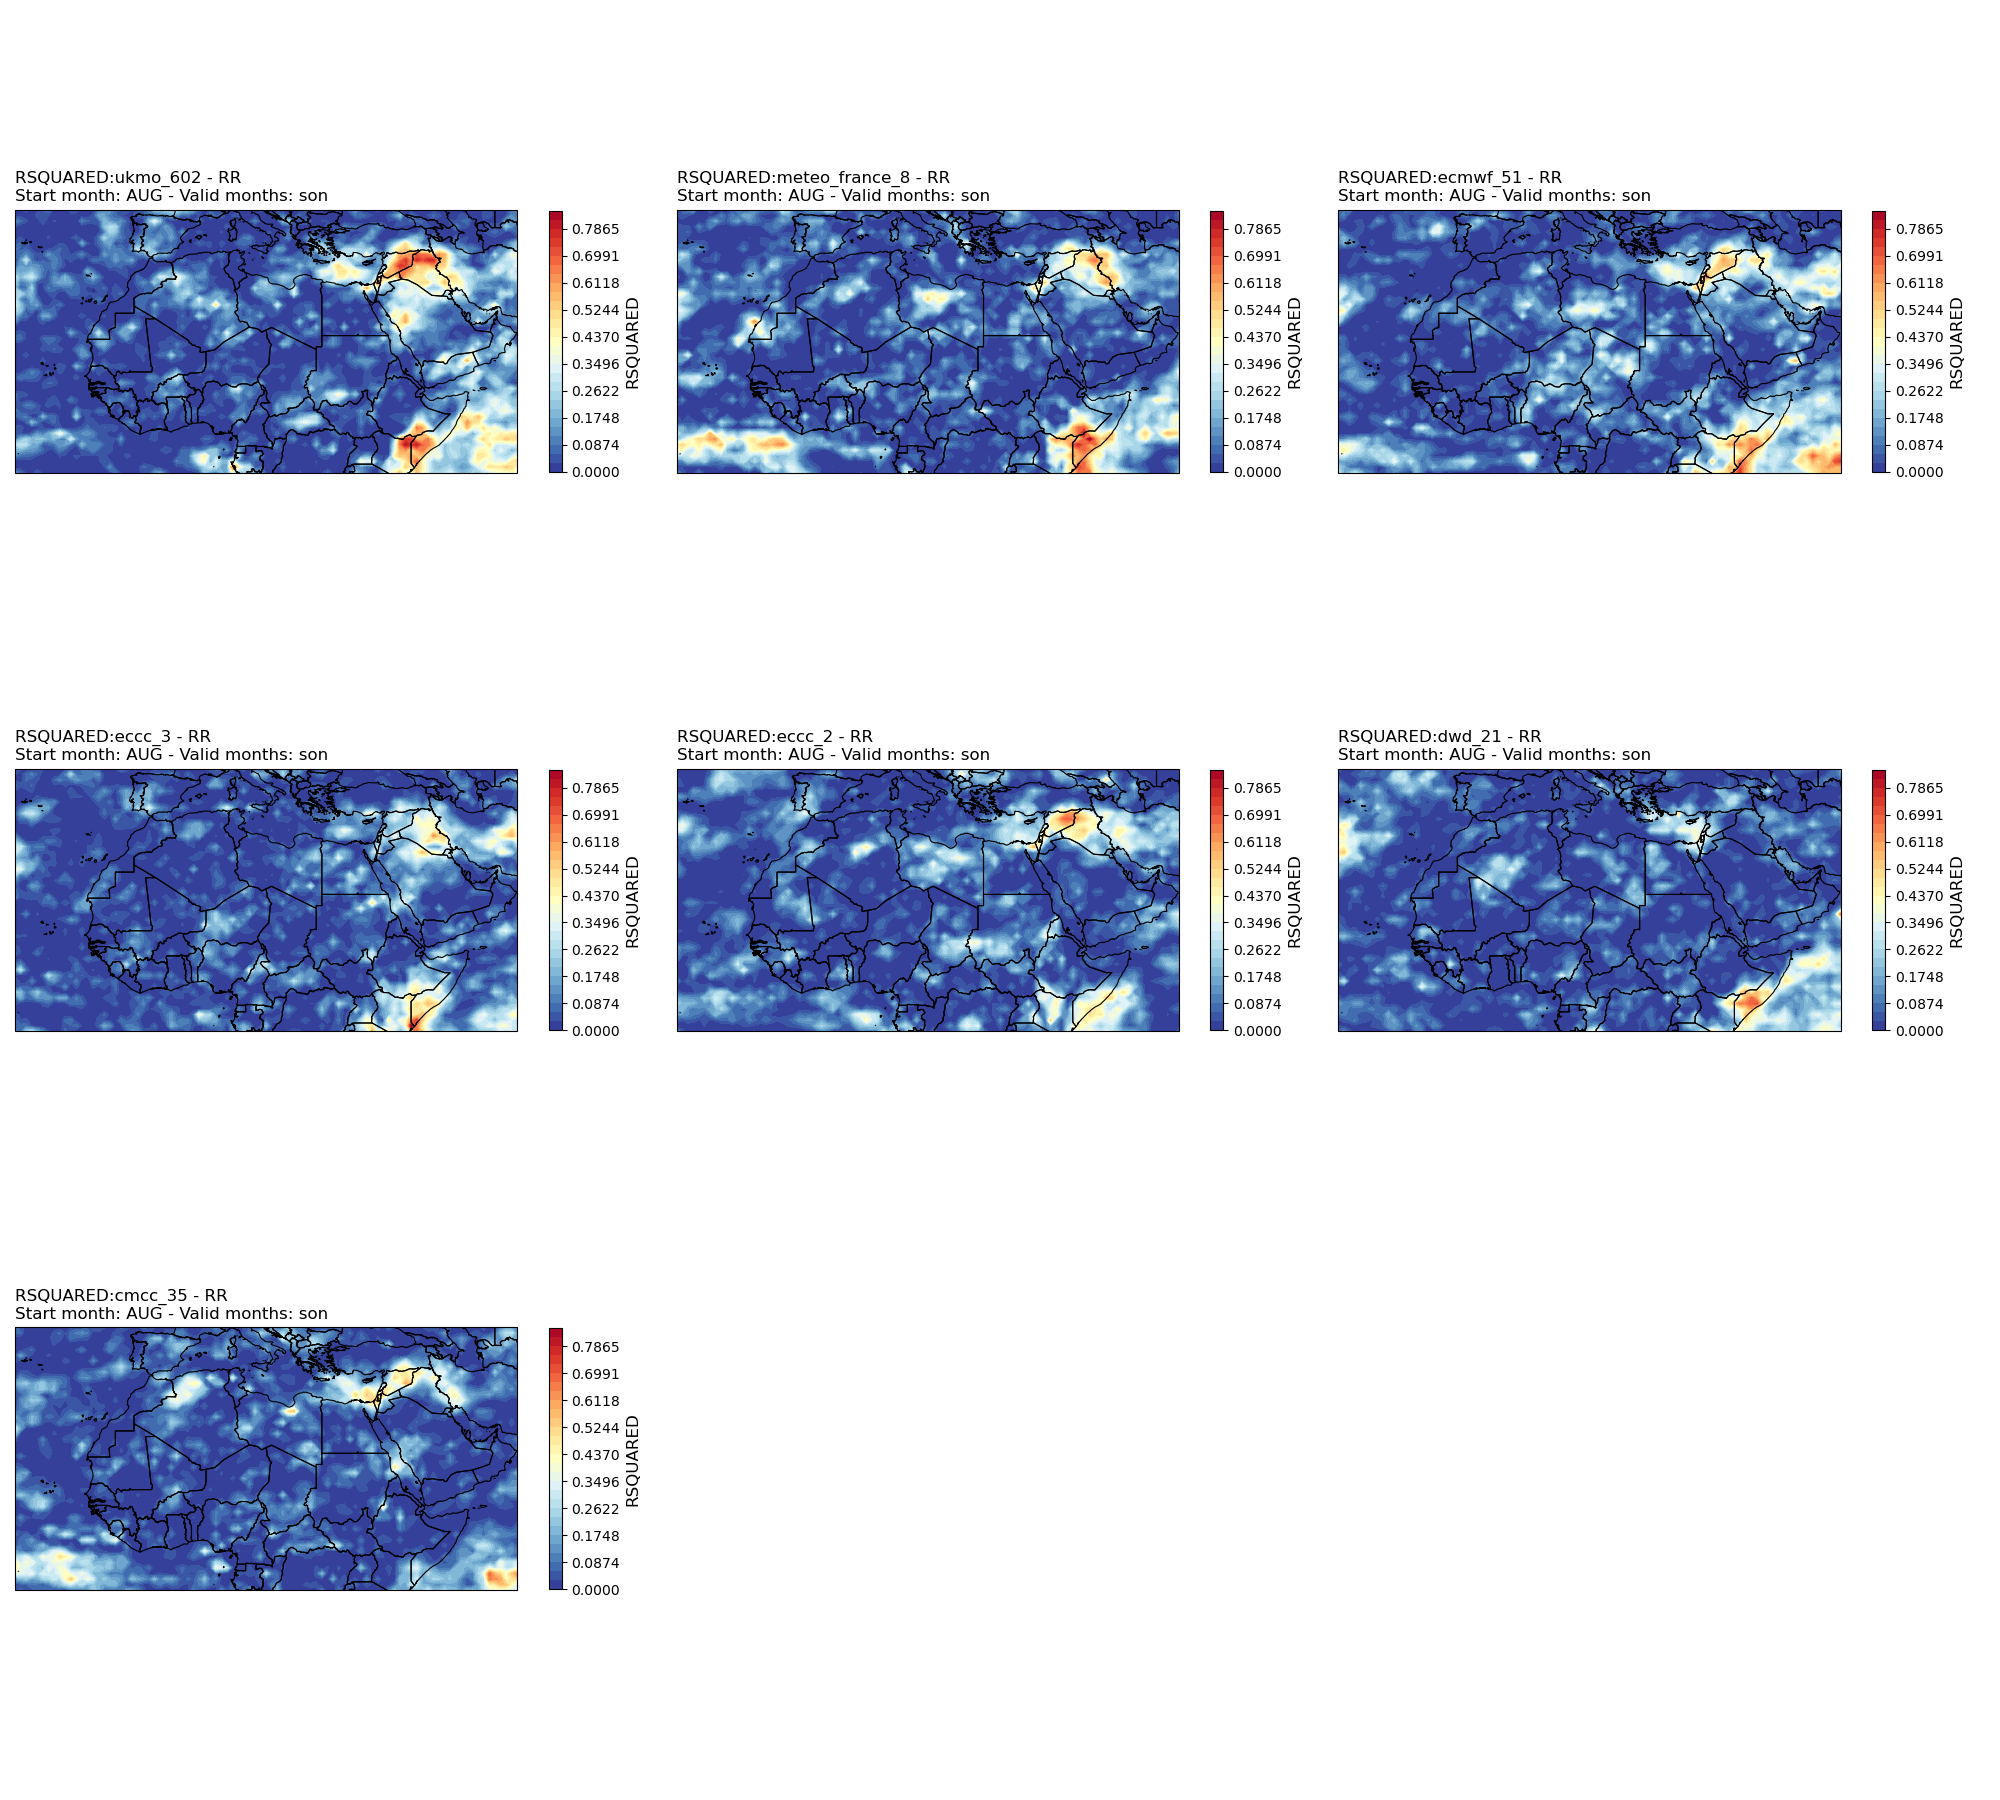
\includegraphics[scale=0.3]{plots/det/rsquared/rsquared_son_RR.png}
\caption{3-months Rolling mean of RSQUARED in MENA Region for all centers SON}
\end{figure}

there is some isolated zones where the r-squared is good especially in Syria, Irak, Jordan ,Palestine  and East Africa, this high performance is observed in all centers. For the rest of the MENA region the performance is very bad with score near to 0. Hence, there is no constant pattern for the R-SQUARED, the spacial variation is very high for all centers.


\subsection{Probabilistic Evaluation Metrics}

\subsubsection{The Brier Score (BS)}

\begin{figure}[H]
    \centering
    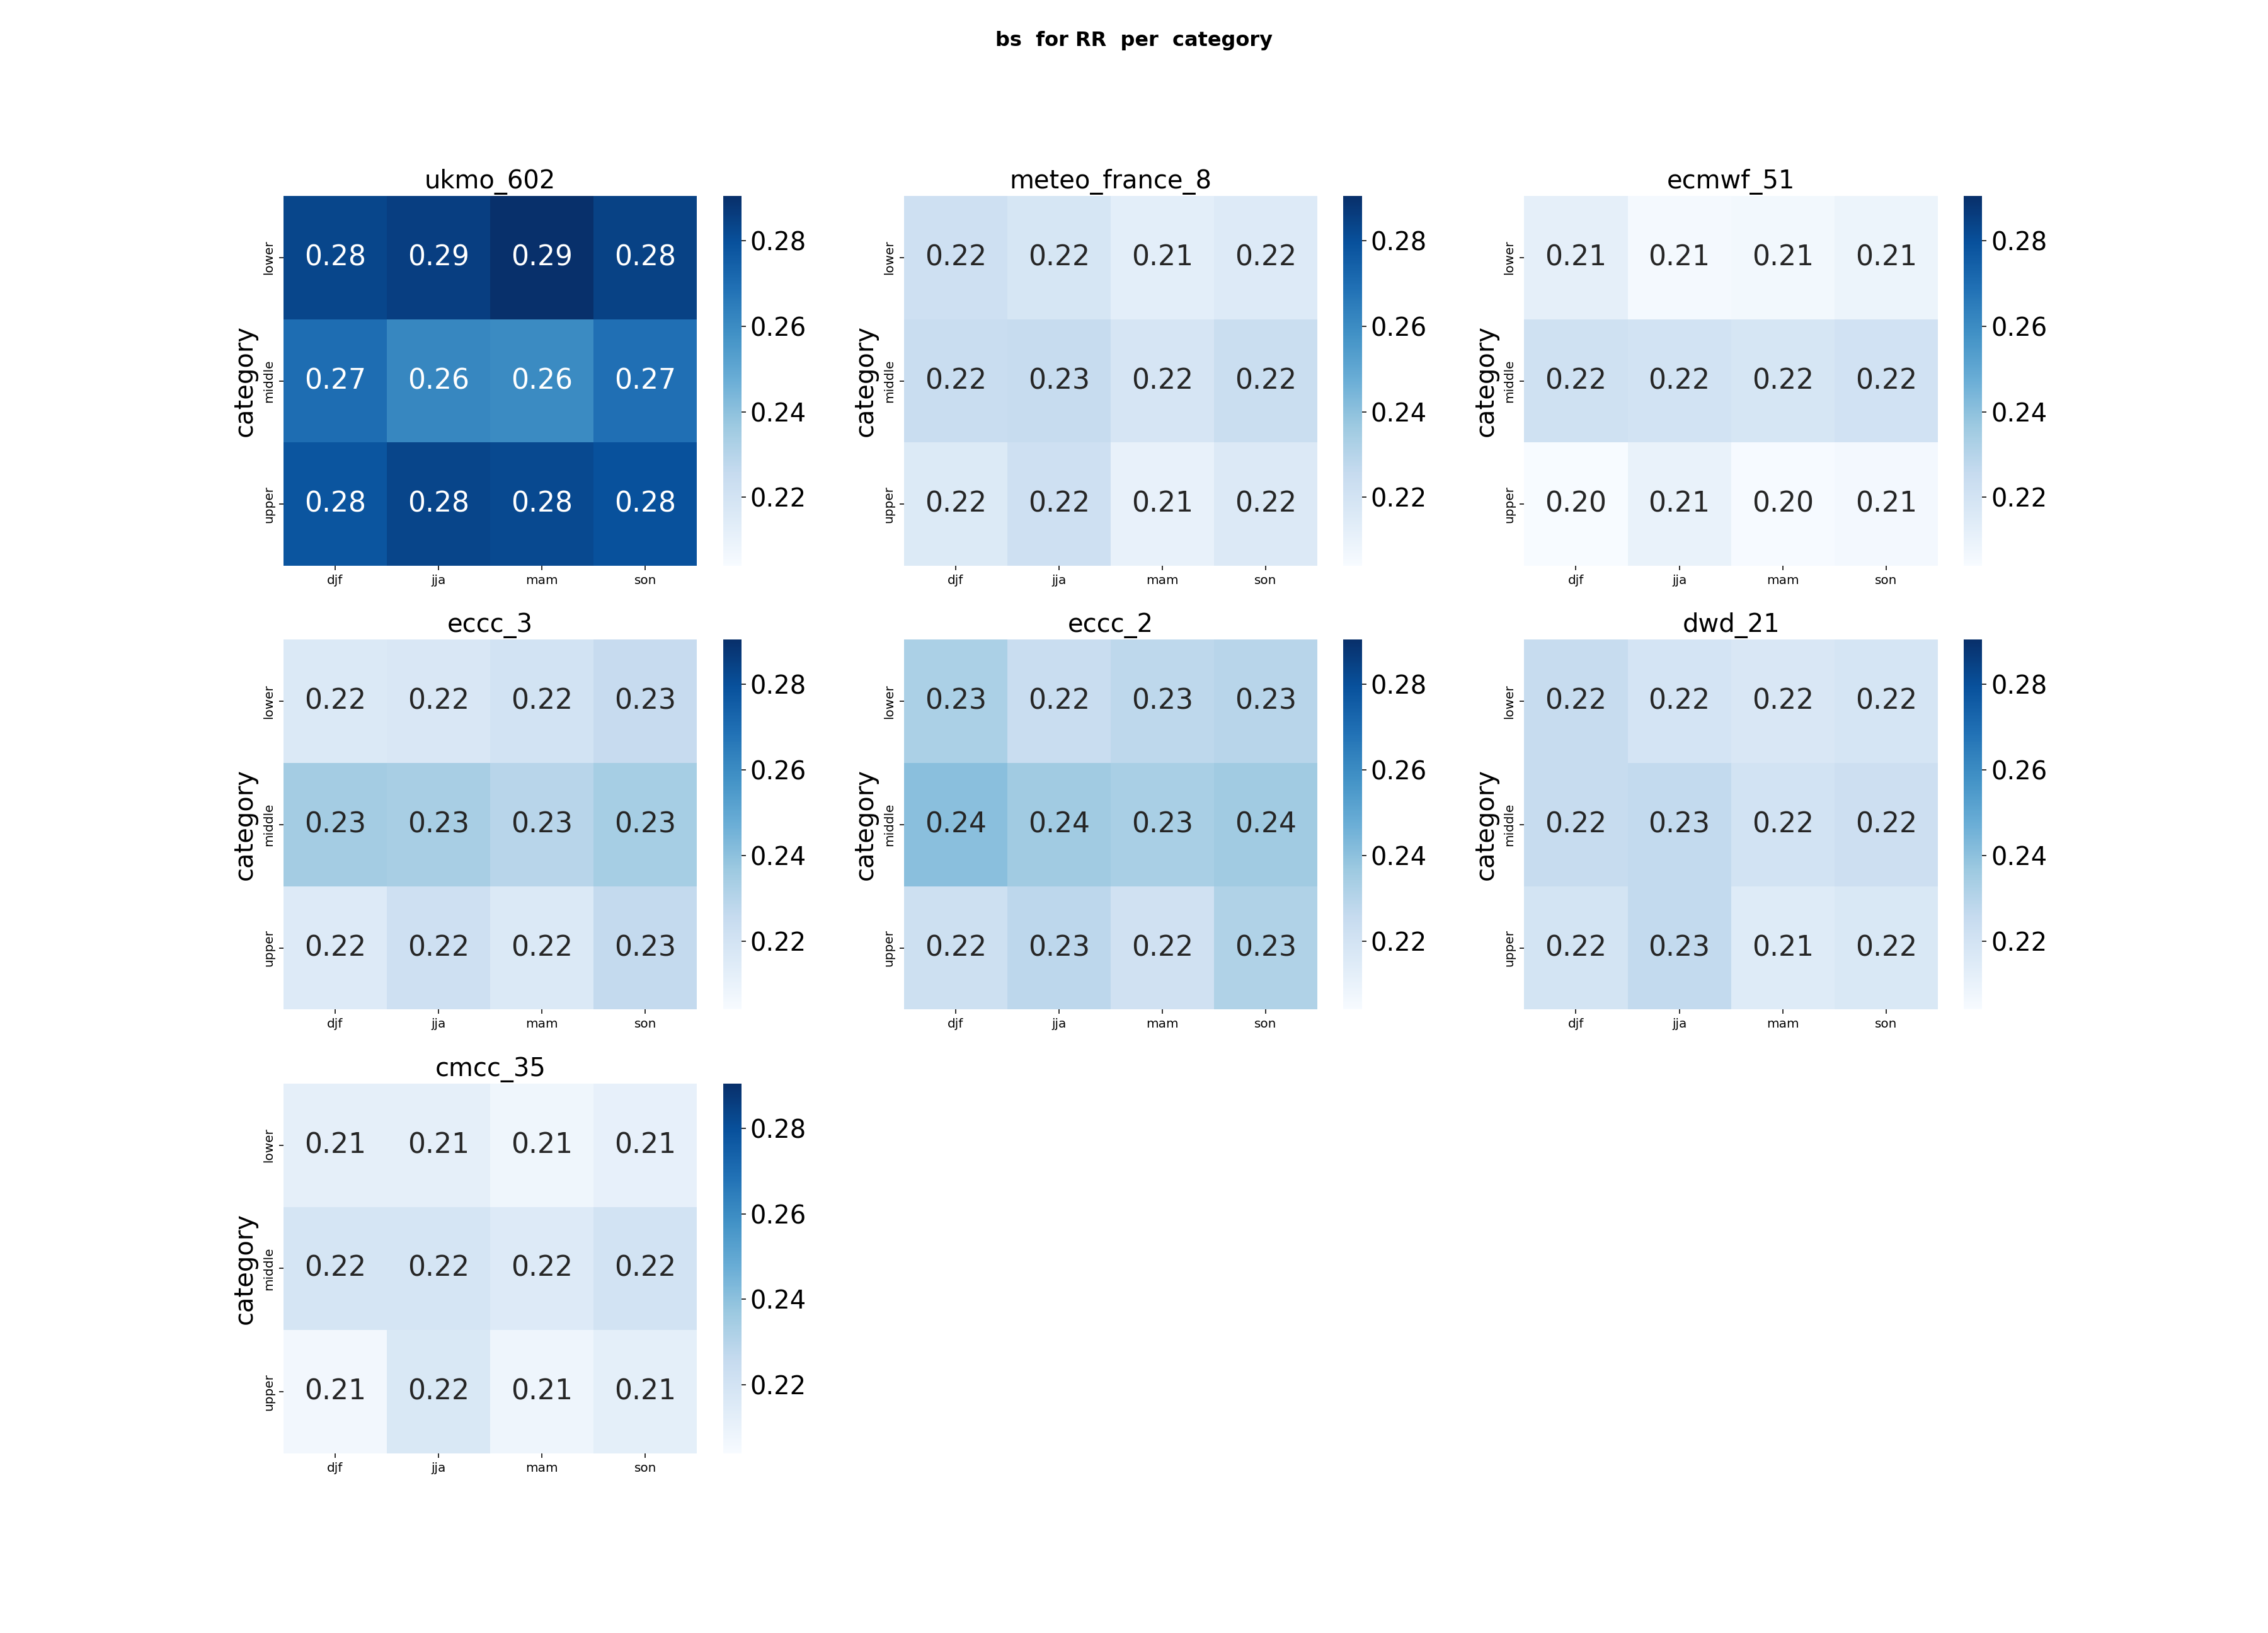
\includegraphics[scale=0.25]{plots/prob/bs/bs_RR_category.png}
    \caption{The Heatmap of Brier Score for each category  . \textbf{\textit{(0 represents perfect BS)}}}
\end{figure}

for the analysis per category, we can see in the figure above that all centers exhibit good performance in term of Brier Score except the UMKO that shows moderate BS. Overall, the middle tercile shows lower performance (higher Brier Score) for all centers. 
the figure below shows the analysis per lead-time. the same result is found, but the \textbf{\textit{ECMWF,METEO-FRANCE and CMCC-35}} are the best models in Brier Score for lead-time analysis.The performance stay stable along time which is a reliable signal. Despite the UKMO have the lower performance, it stays close to the other centers, the difference isn't so wide. 
In general, the performance stays stable over category, lead-time and space.


\begin{figure}[H]
    \centering
    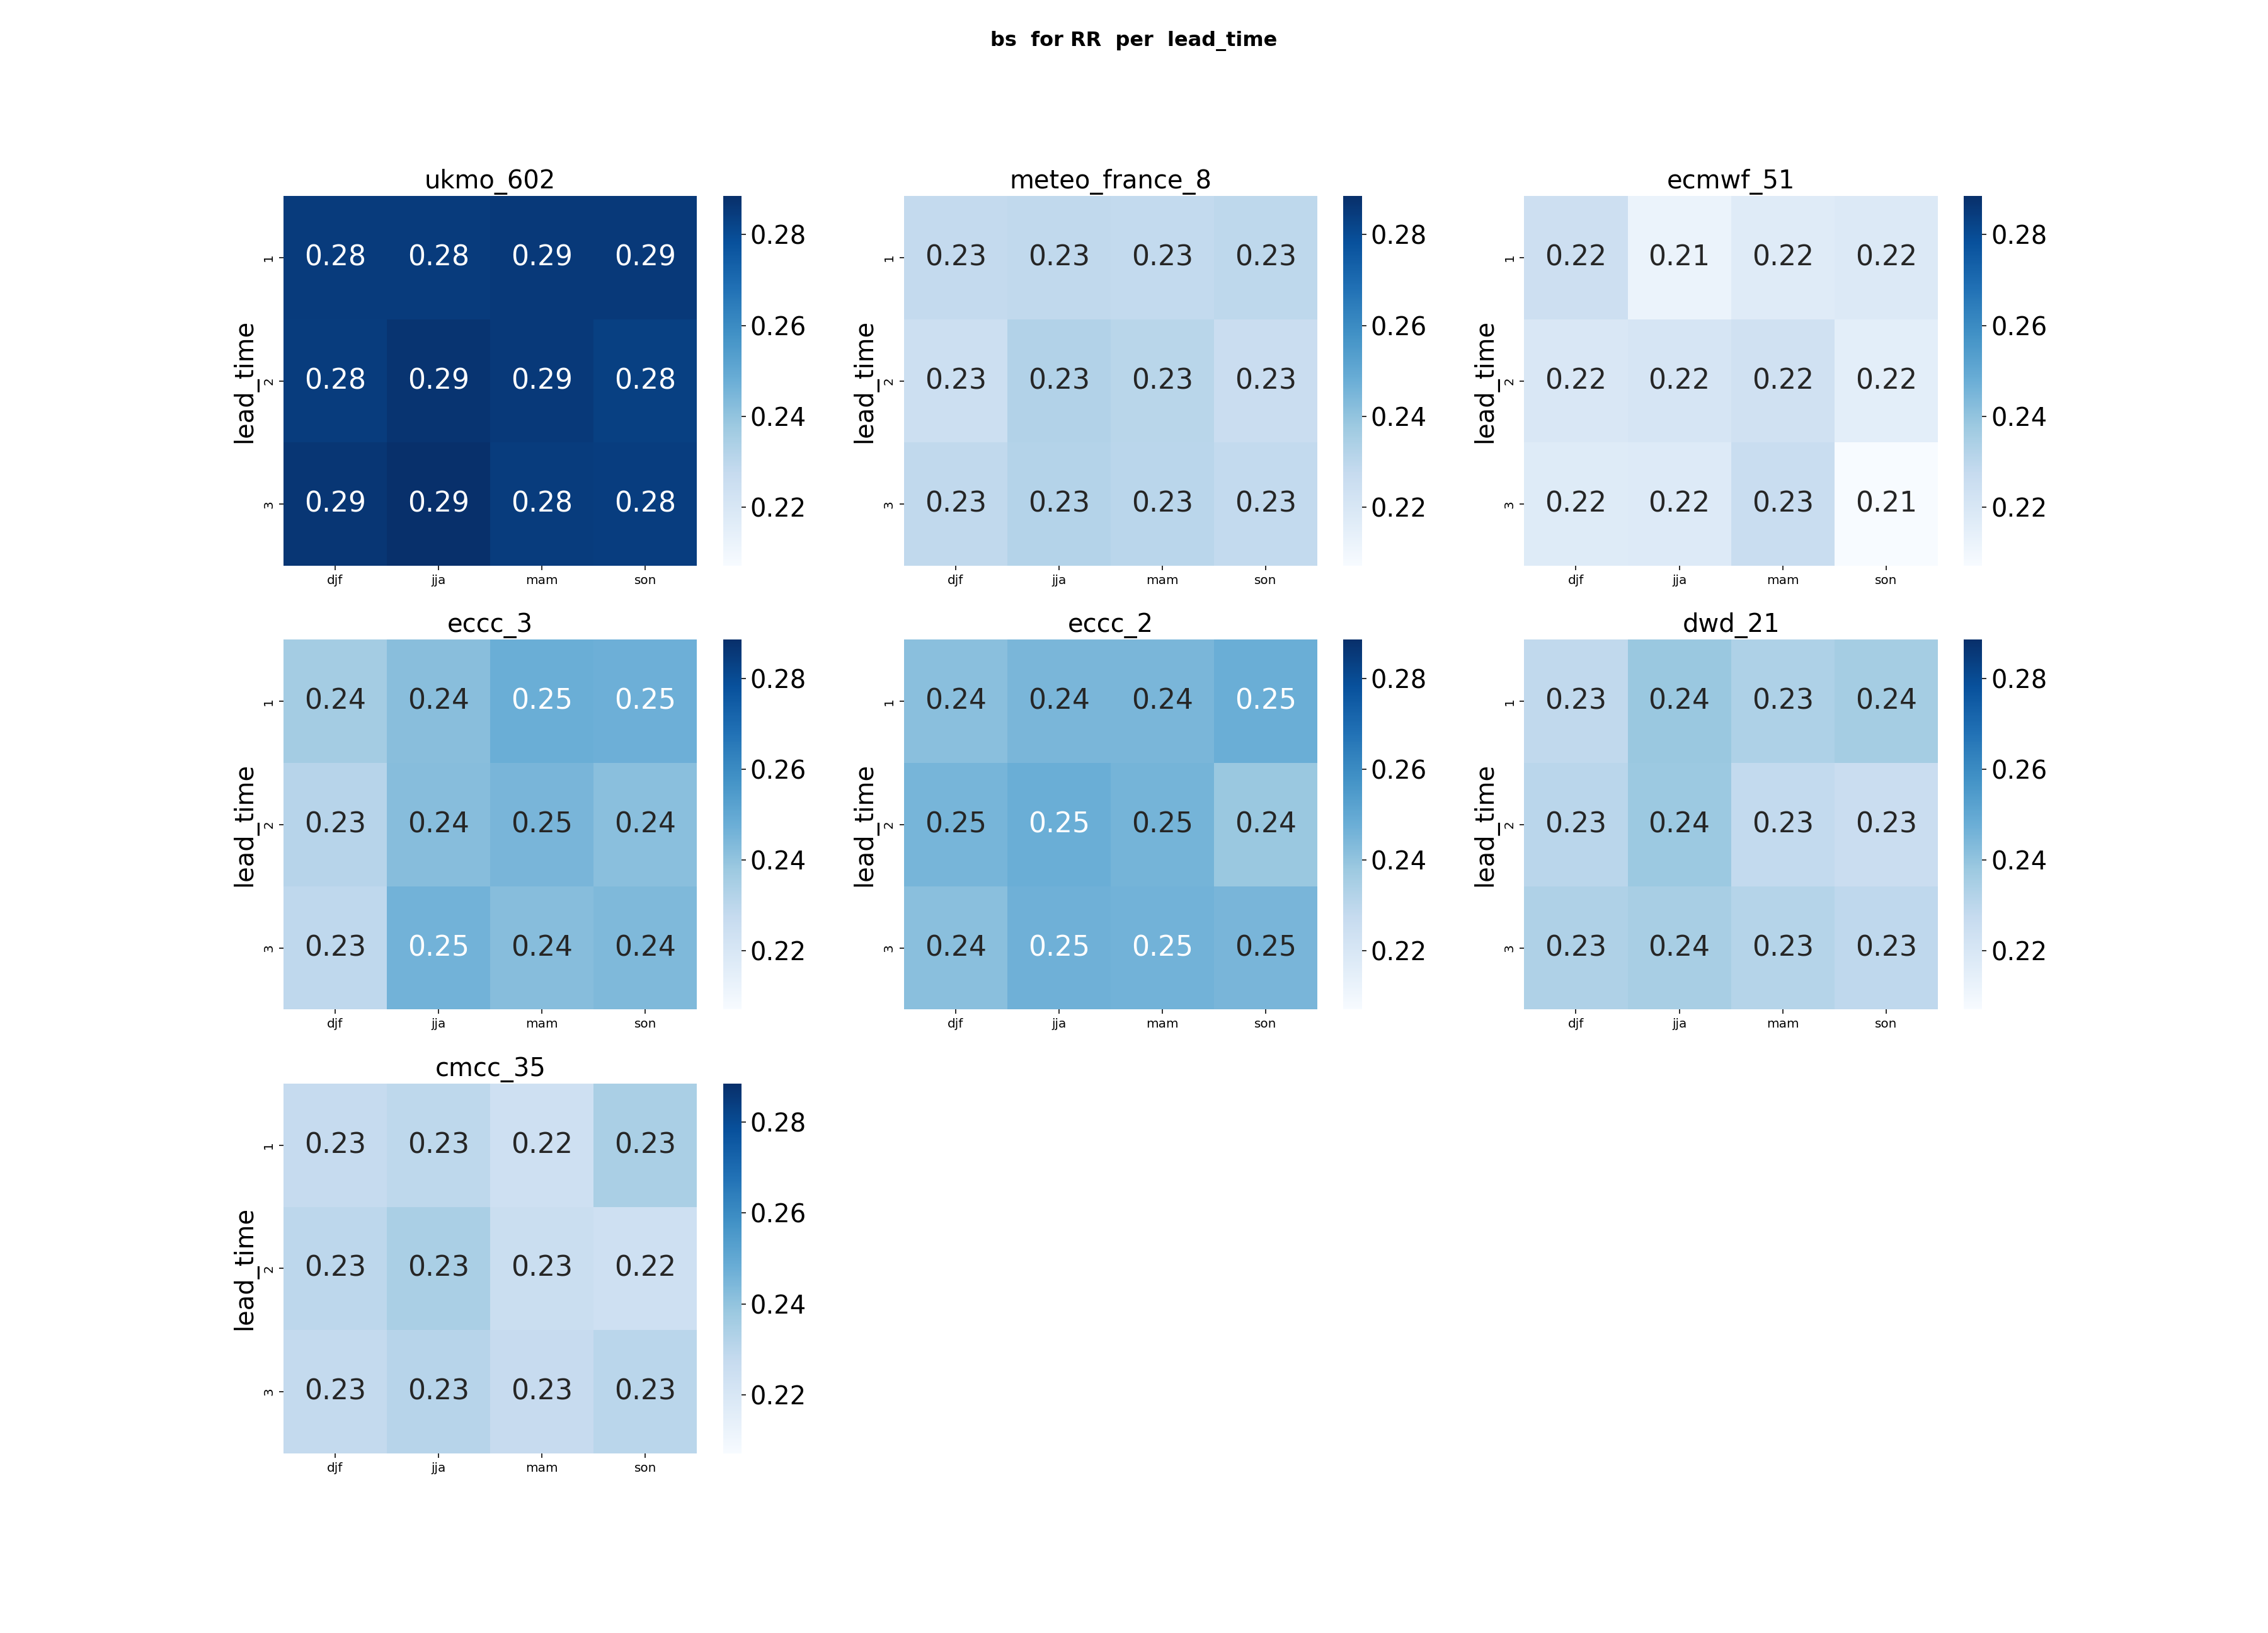
\includegraphics[scale=0.25]{plots/prob/bs/bs_RR_lead_time.png}
    \caption{The Heatmap of Brier Score for lead-time. \textbf{\textit{(0 represents perfect BS)}}}
\end{figure}


\begin{figure}[H]
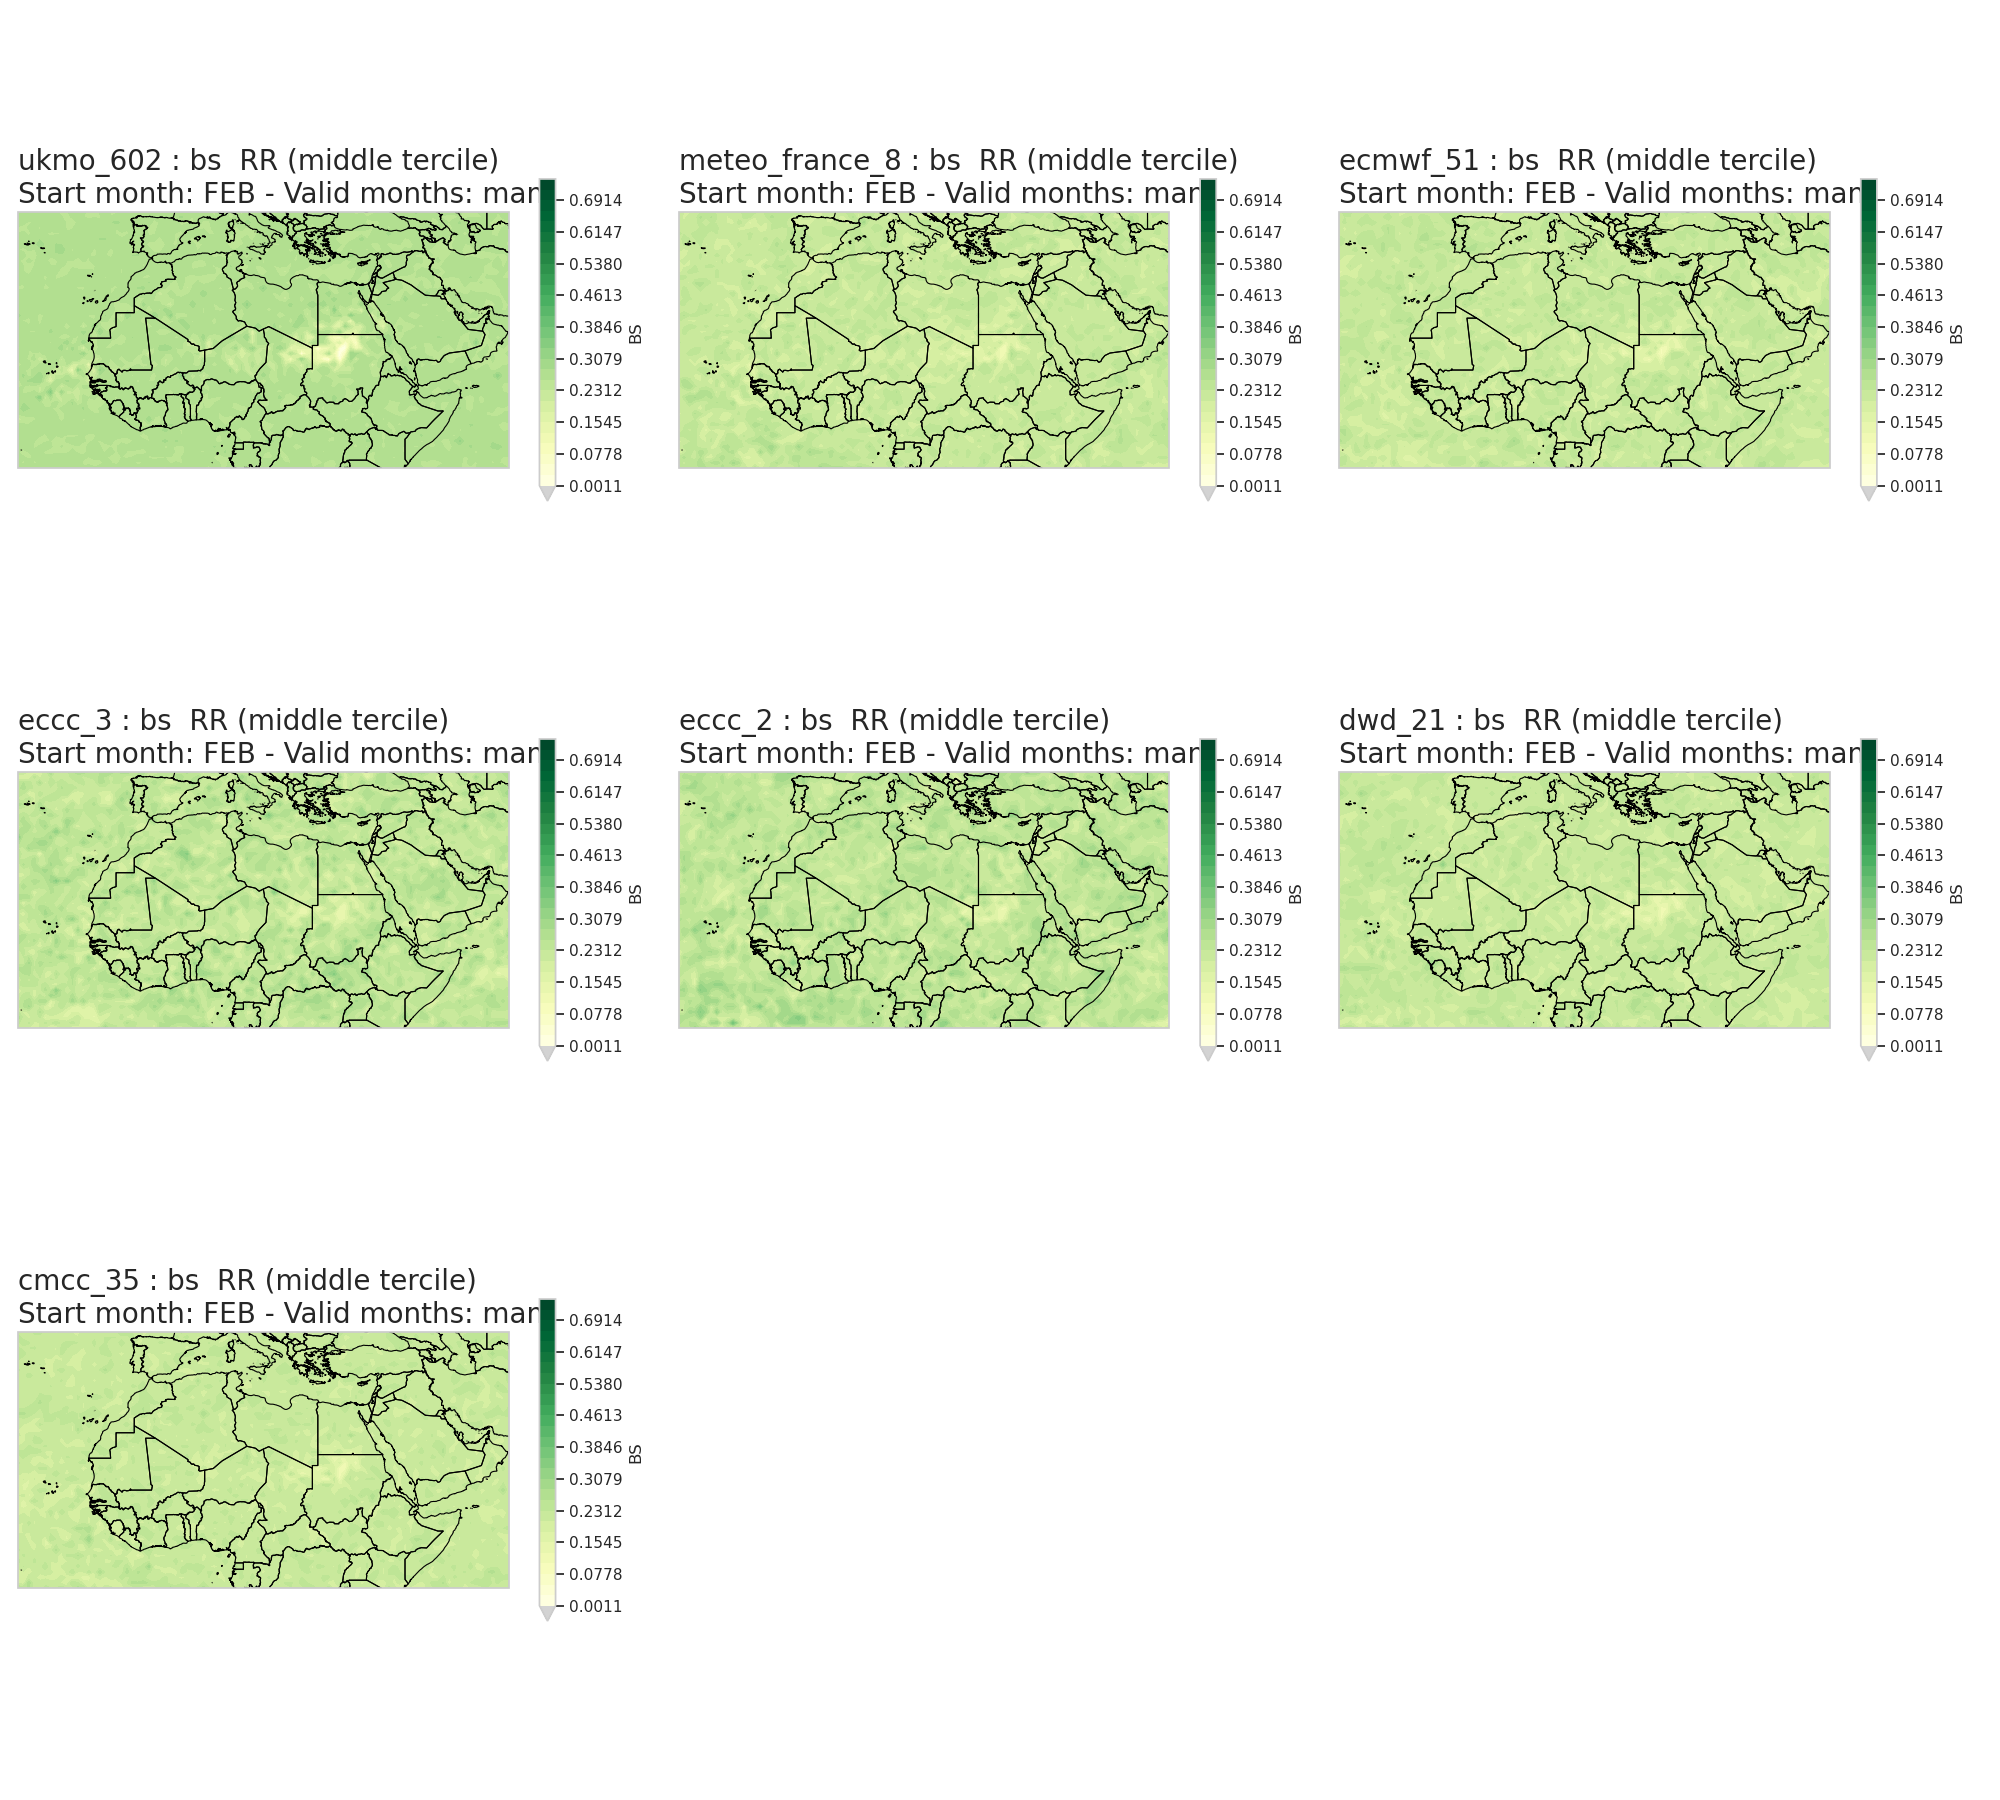
\includegraphics[scale=0.3]{plots/prob/bs/bs_mam_RR_middle.png}
\caption{3-months Rolling mean of Brier Score in MENA Region for all centers middle tercile MAM}
\end{figure}

the spacial distribution of the BS is homogeneous, the same performance across the MENA region, almost all centers perform well for all lead-times, for  tercile there is a little lower performance for the middle tercile.
Hint, for the other seasons the results are almost the same. 


\subsubsection{Reliability}

\begin{figure}[H]
    \centering
    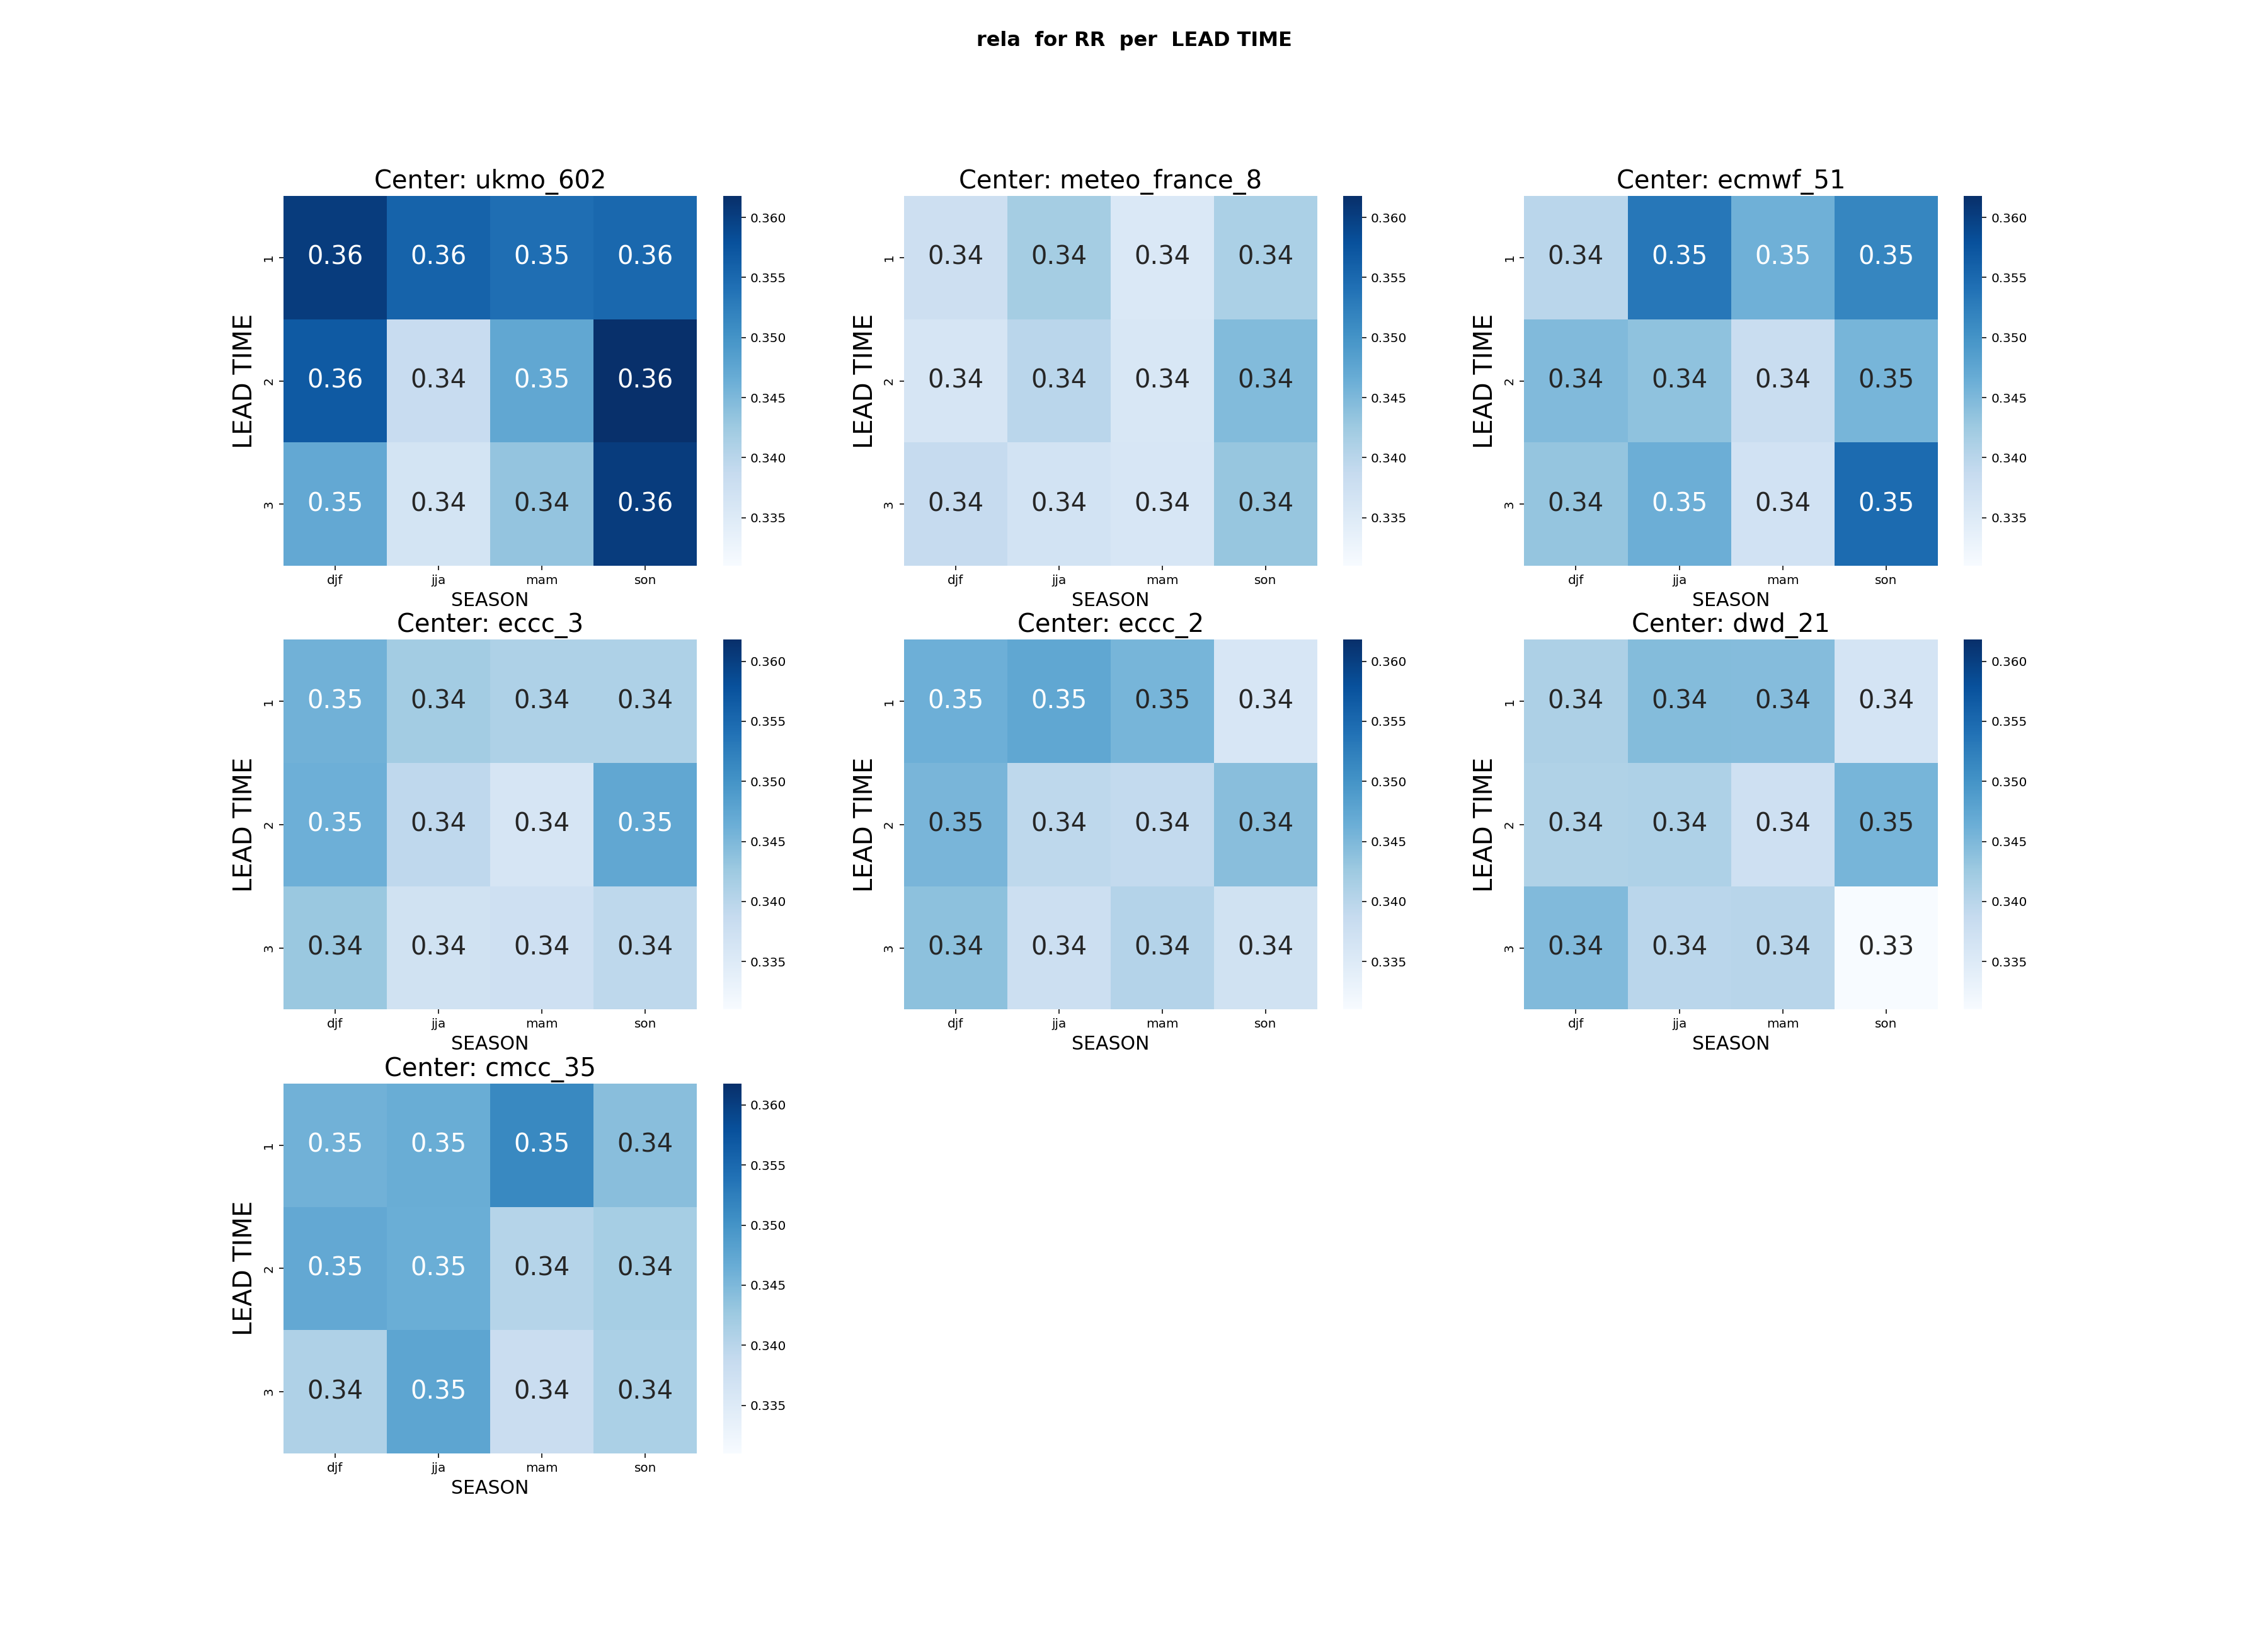
\includegraphics[scale=0.25]{plots/prob/rela/rela_RR.png}
    \caption{The Reliability Score  . \textbf{\textit{(0 means perfect Reliability)}}}
\end{figure}

In the figure above, all centers demonstrate similar moderate performance in term of reliability. But deep analysis within the figure below, shows that UKMO has very bad performance, also we can distinguish three models that have the best reliability according to the reliability diagram, the centers are \textbf{\textit{ECMWF,CMCC and METEO-FRANCE}}. Hence,all centers give similar description of the reliability, also the stability along lead-time is a good indicator despite of the moderate results (0.3), we can rely on the models cited above because of the acceptable results and the stability along time.

\begin{figure}[H]
\centering
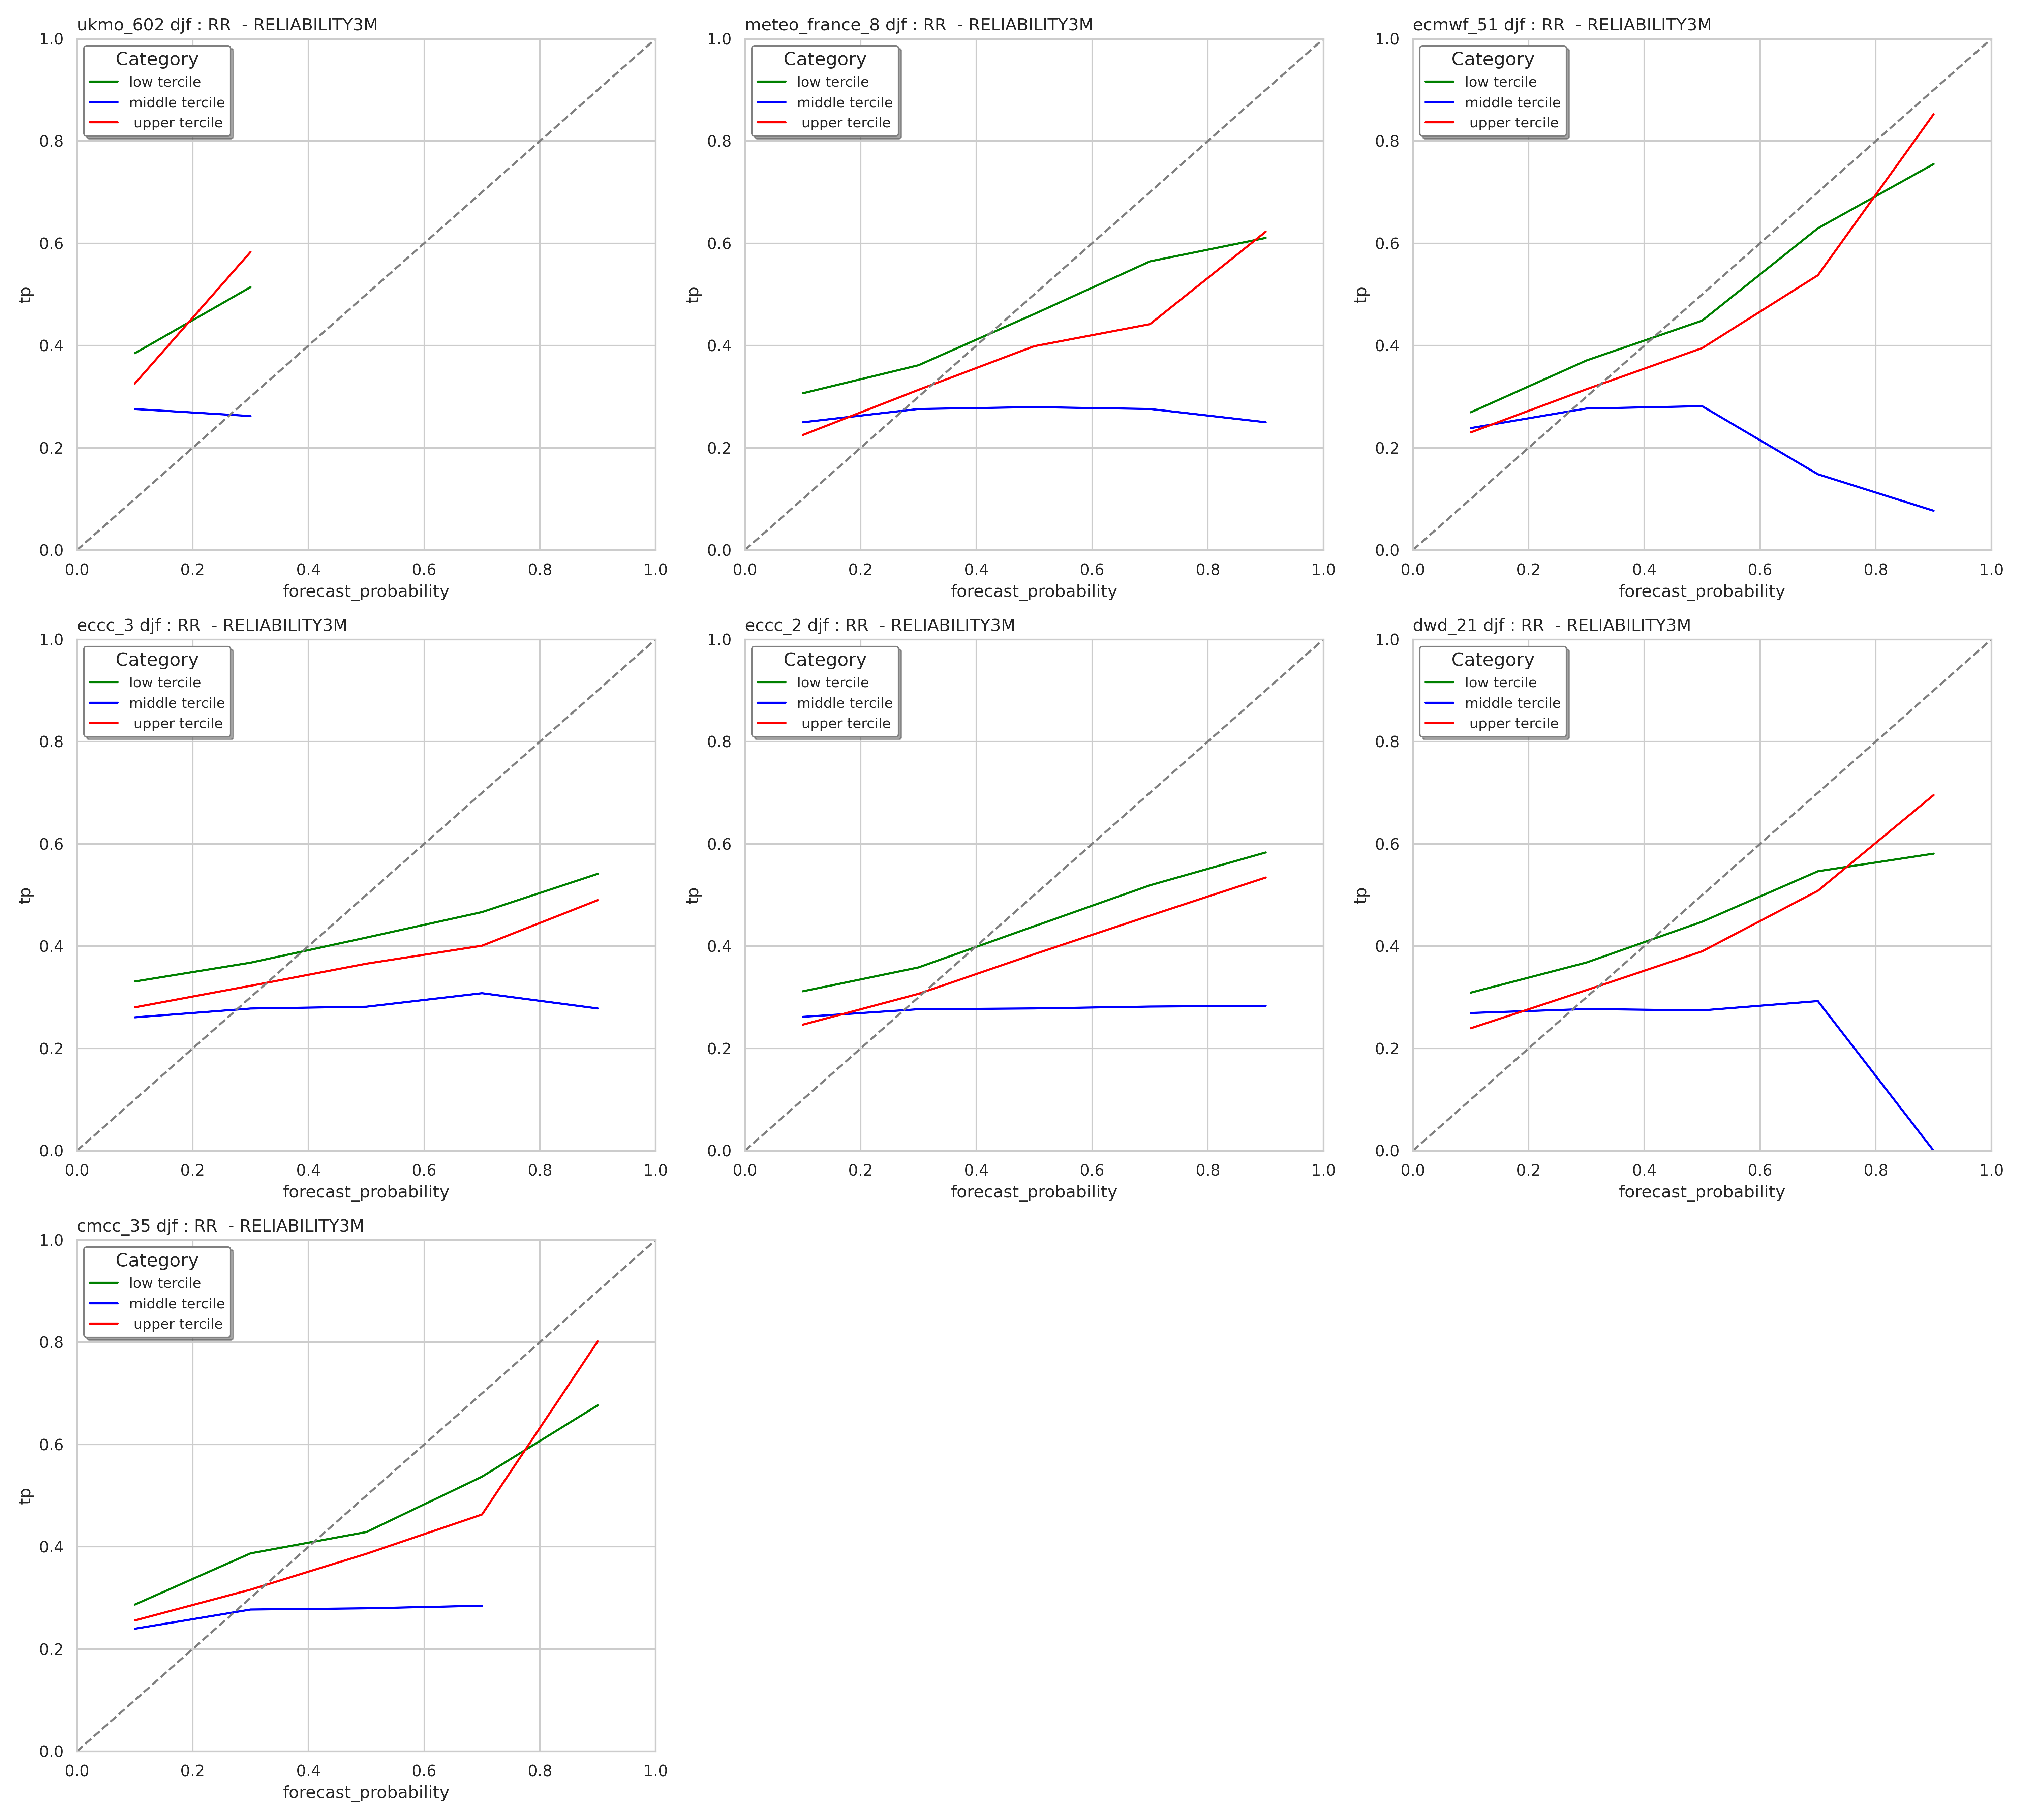
\includegraphics[scale=0.3]{plots/prob/rela/rela_diagram_RR_djf.png}
\caption{The 3-month rolling mean for Reliability DJF   . \textbf{\textit{Reliability is better in cases where the graphs are closer to the 45-degree line}}}
\end{figure}

for the reliability diagram, all centers show moderate results, except for the ukmo that shows lower reliability.Thus, for the lower and upper terciles, models in general show good reliability, but for the middle tercile, this models aren't reliable. above all, \textbf{\textit{ecmwf}}  shows the highest performance for reliability.


\subsubsection{The ranked probability score (RPS)}


\begin{figure}[H]
    \centering
    \includegraphics[scale=0.25]{plots/prob/rps/rps_RR.png}
    \caption{The Heatmap of  RPS Score on MENA region for Precipitations    . \textbf{\textit{(0 means perfect RPS)}}}
\end{figure}

In the figure above, all centers demonstrate moderate performance, except for UKMO, which shows noticeably lower performance. 


\begin{figure}[H]
    \centering
    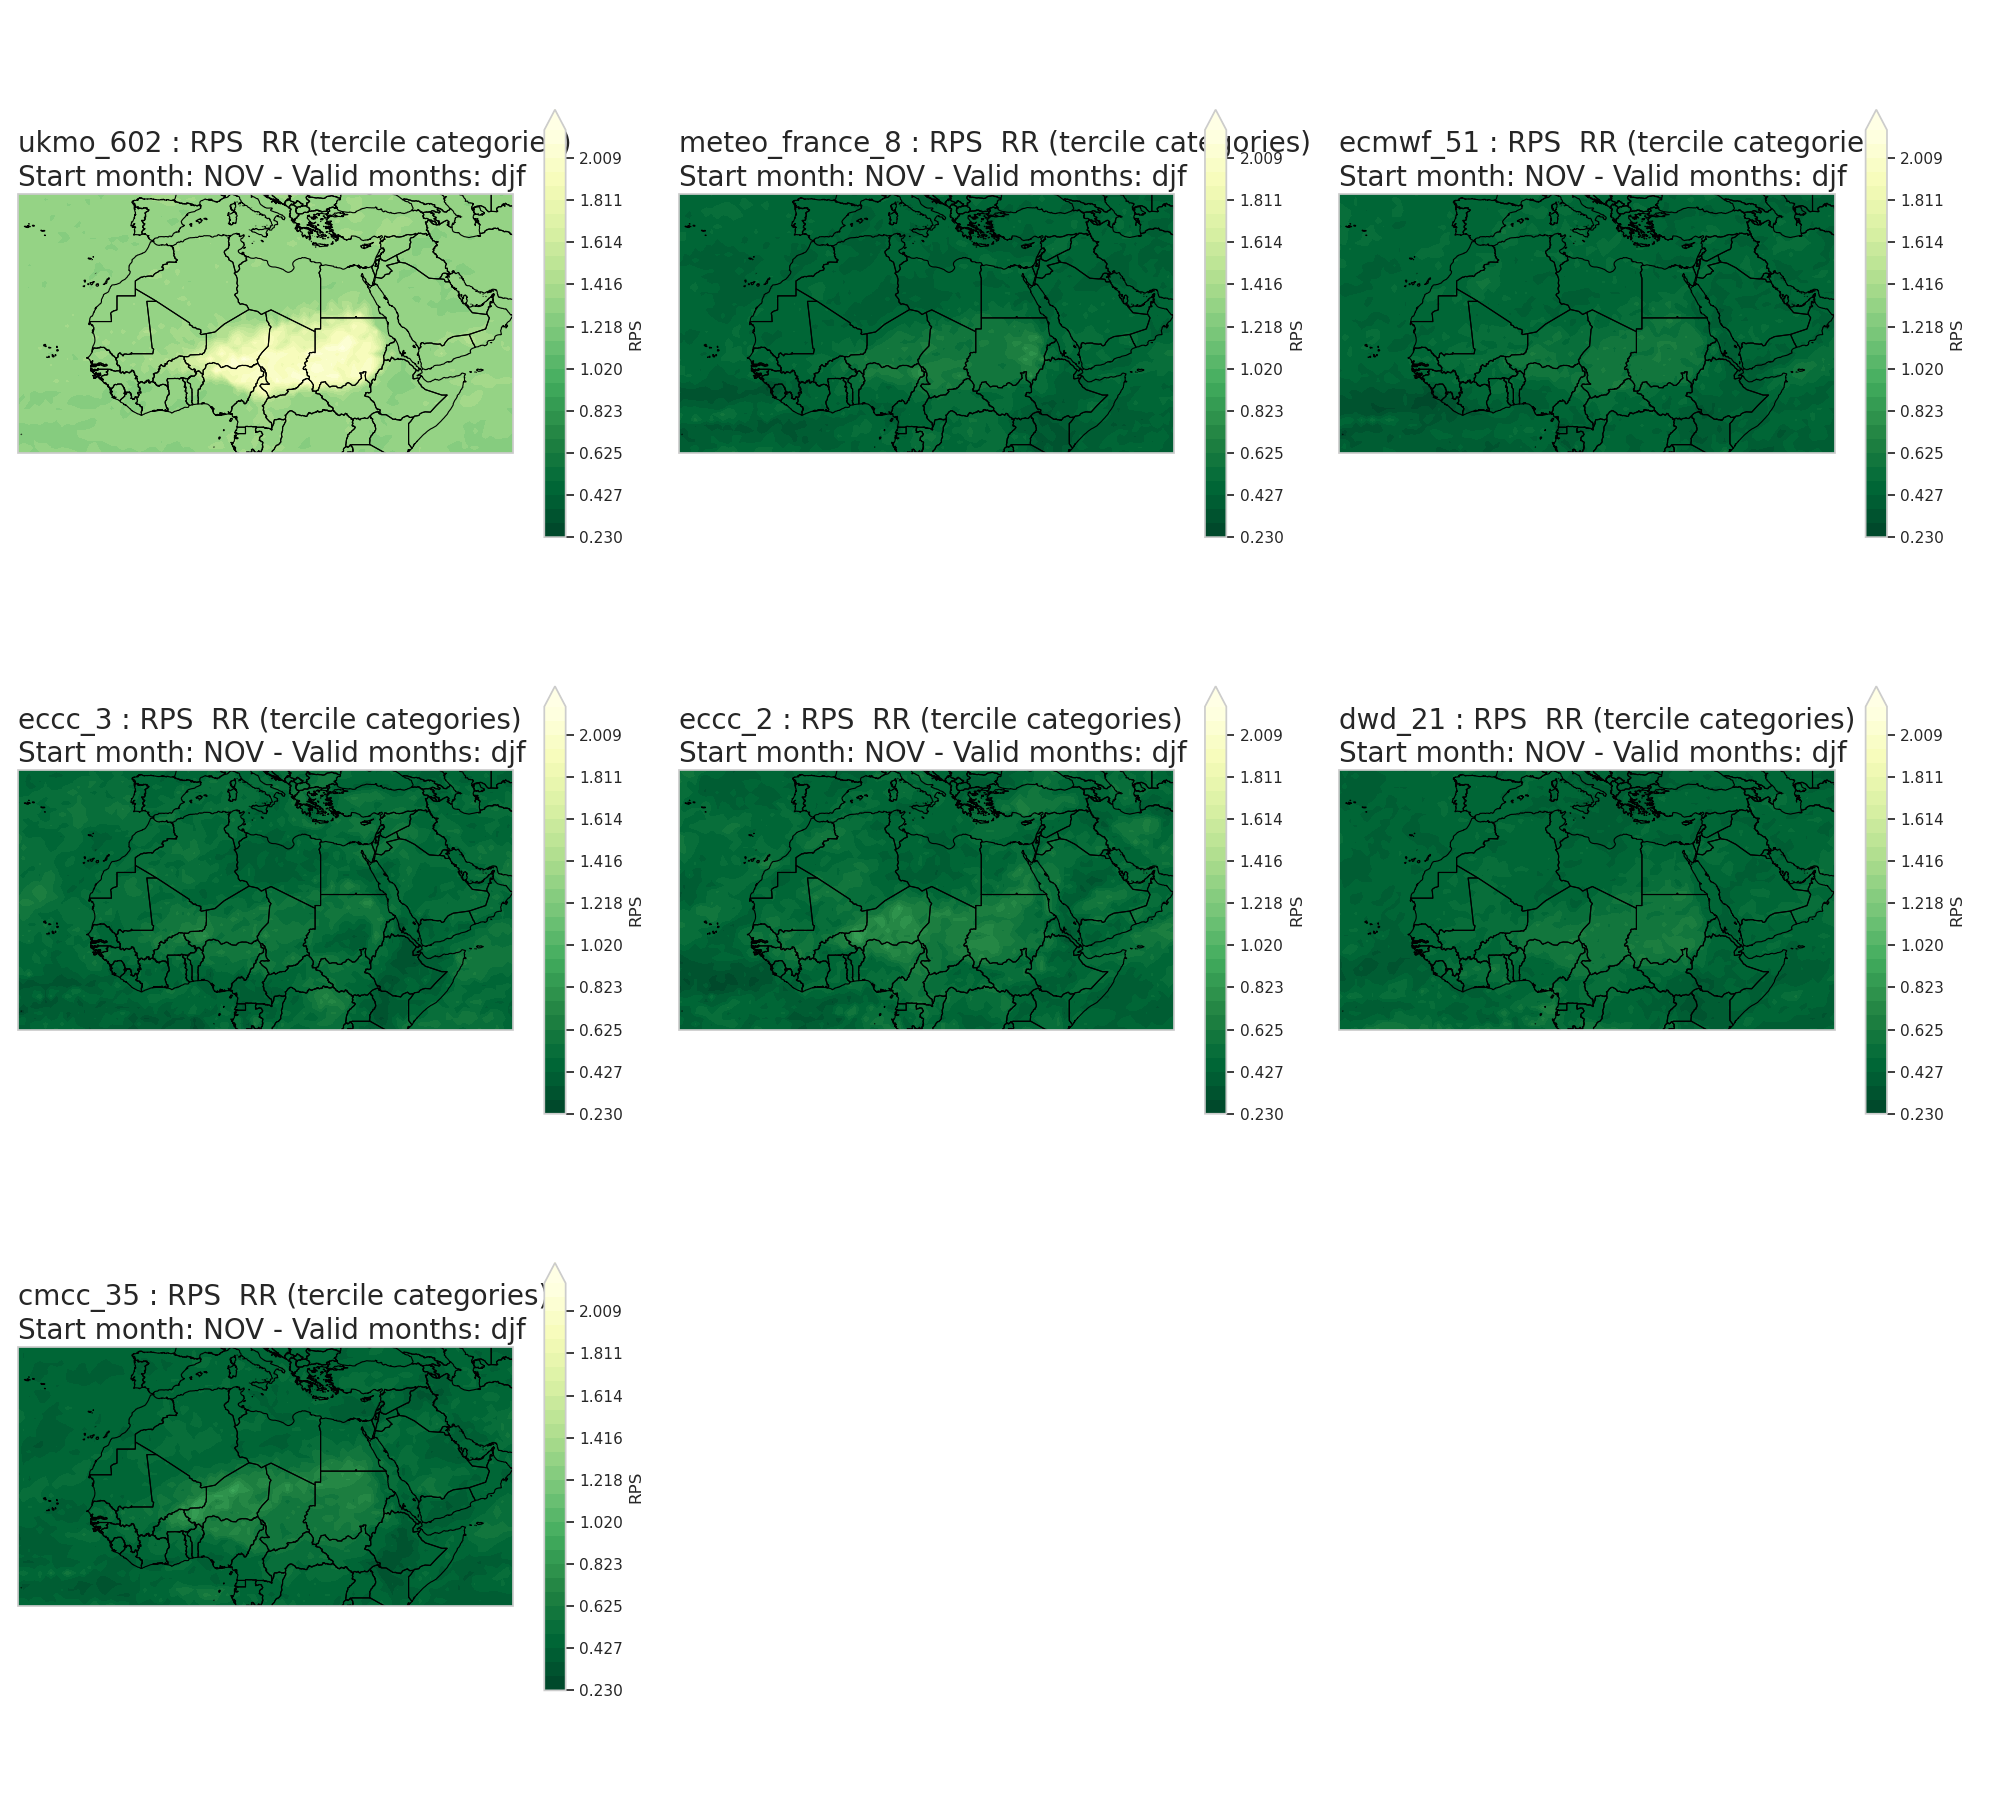
\includegraphics[scale=0.25]{plots/prob/rps/rps_djf_RR.png}
    \caption{The   RPS Score on MENA region for Precipitations DJF   . \textbf{\textit{(0 means perfect RPS)}}}
\end{figure}

the spacial distribution of the RPS, is homogeneous, in all the region the score is good for all centers.Thus, the ukmo shows lower performance for this score.


\subsubsection{Relative operating characteristics}

\begin{figure}[H]
    \centering
    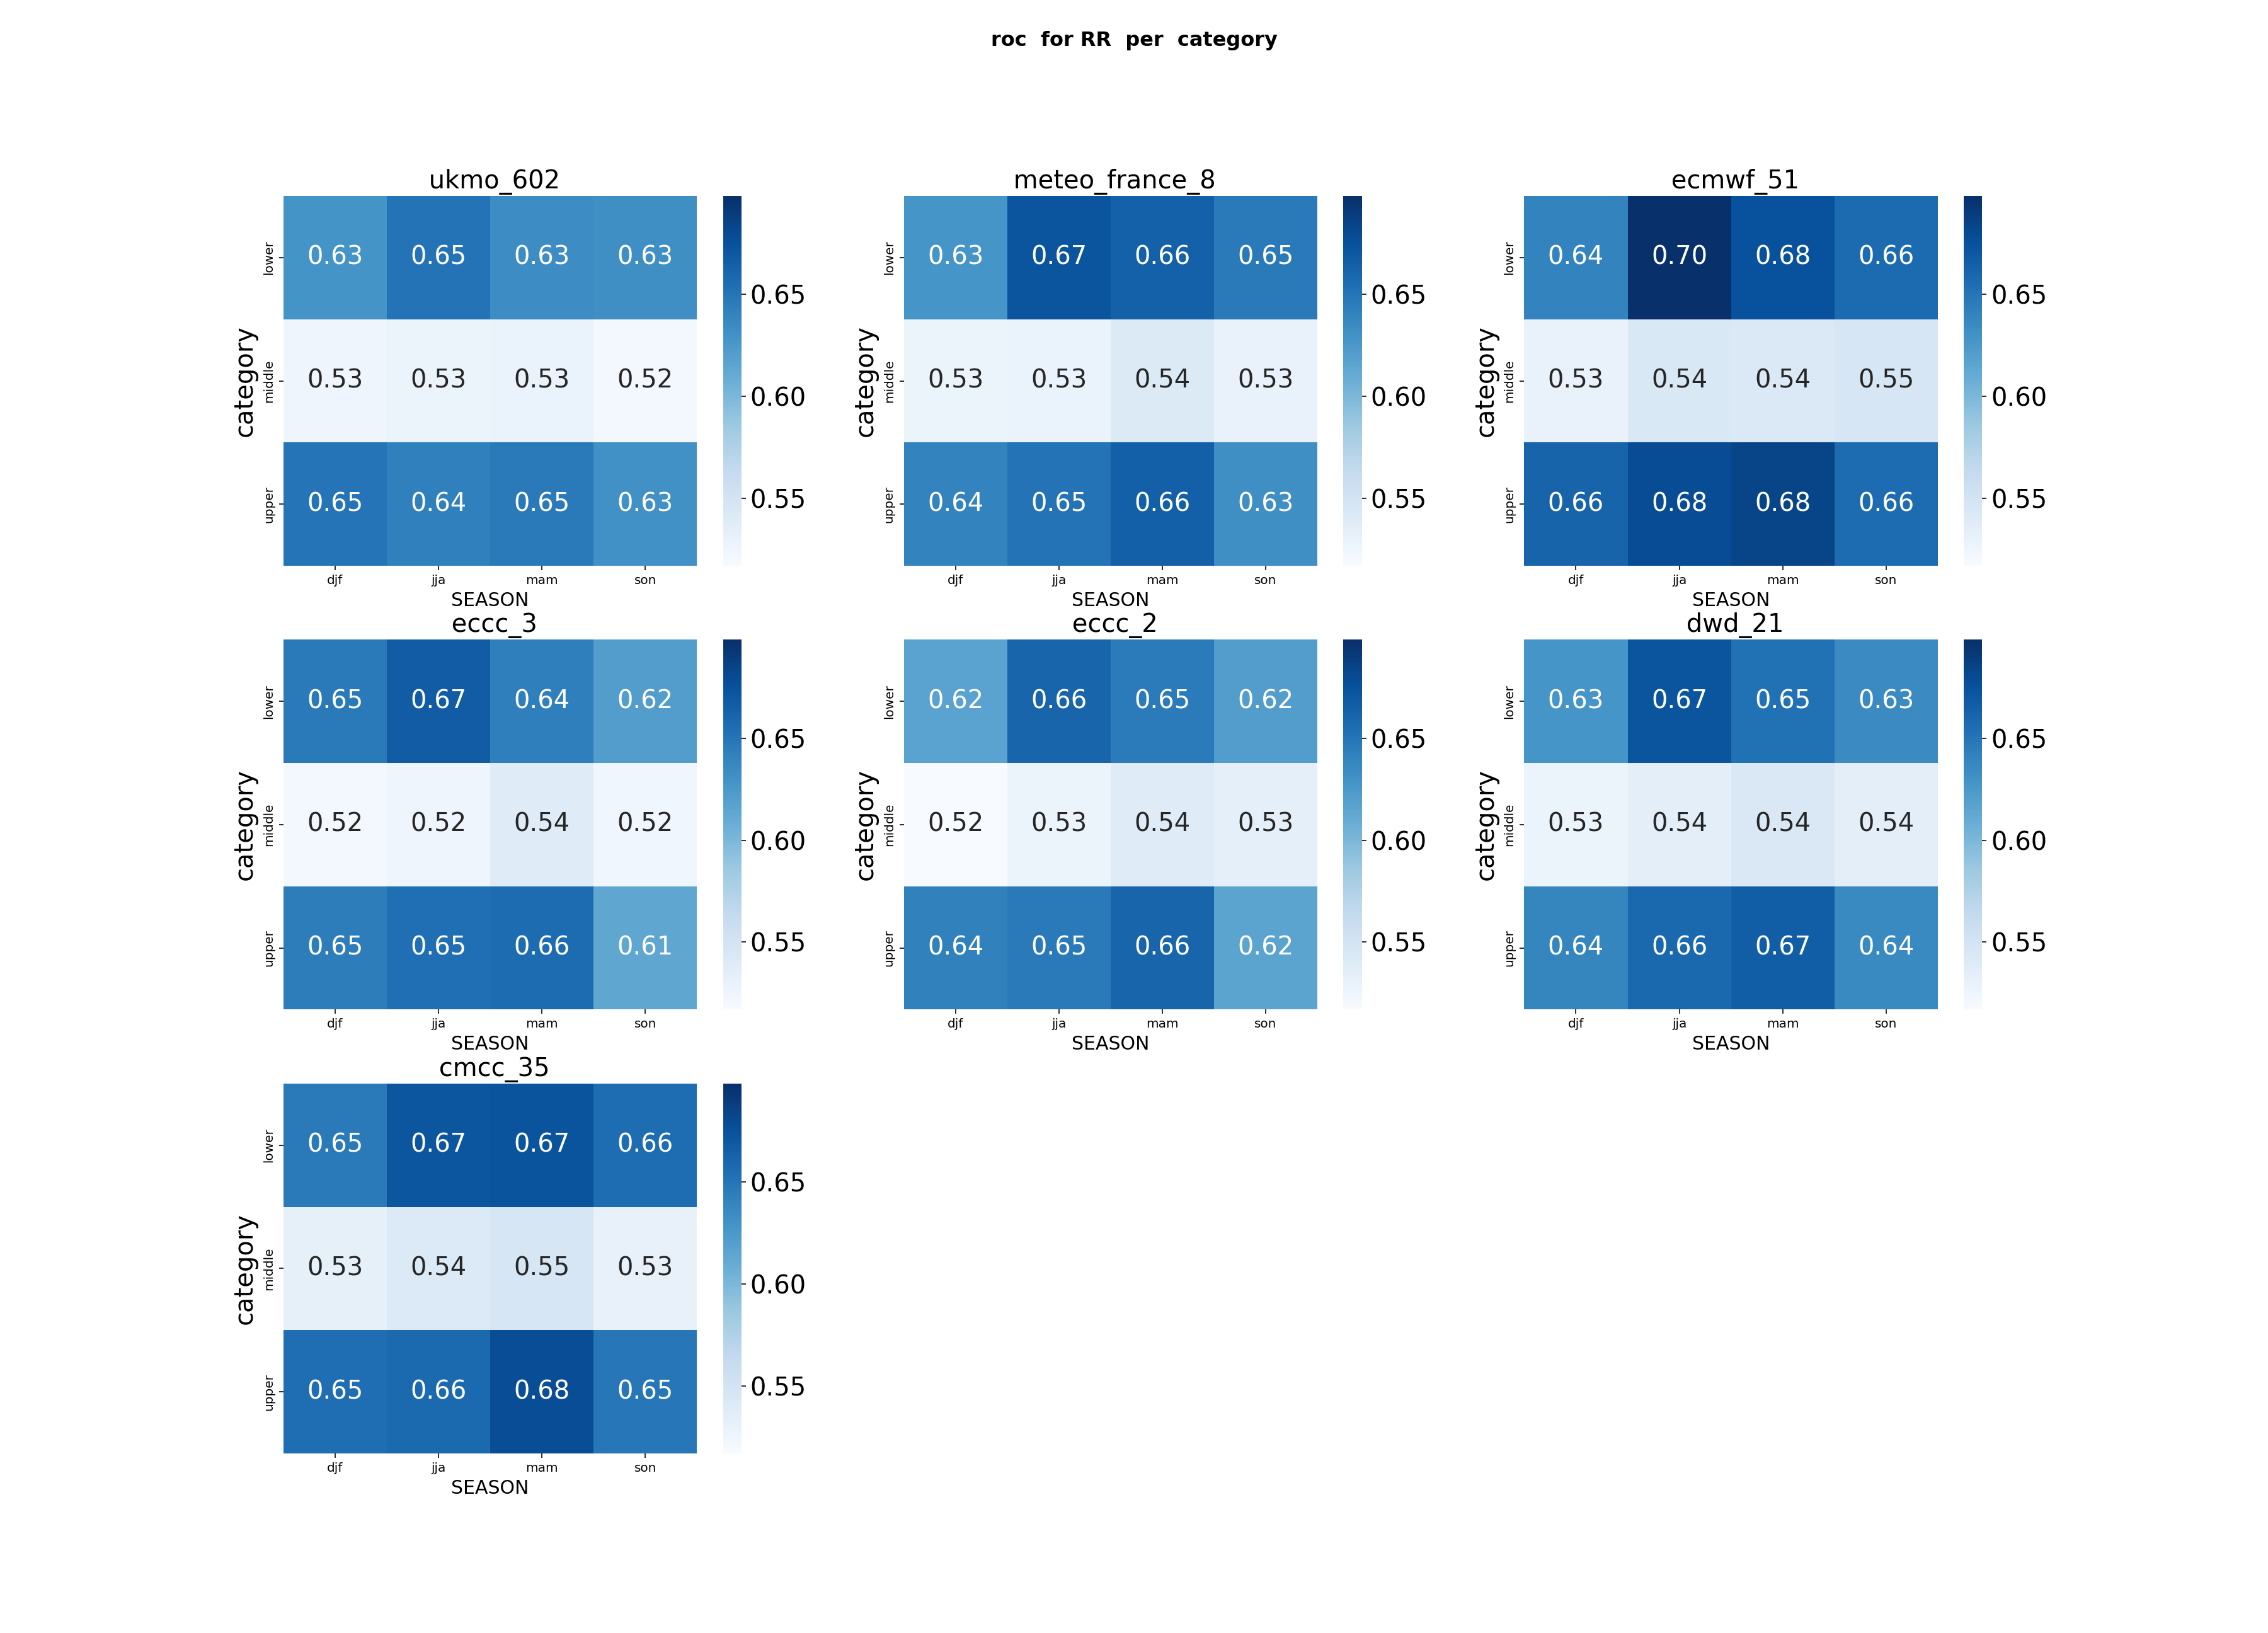
\includegraphics[scale=0.25]{plots/prob/roc/roc_RR_category.png}
    \caption{The Heatmap of ROC Score for each category  . \textbf{\textit{(1 means perfect ROC)}}}
\end{figure}

In the figure above, it is evident that all centers exhibit similar performance levels. However, the middle tercile consistently achieves the lowest score.
\begin{figure}[H]
    \centering
    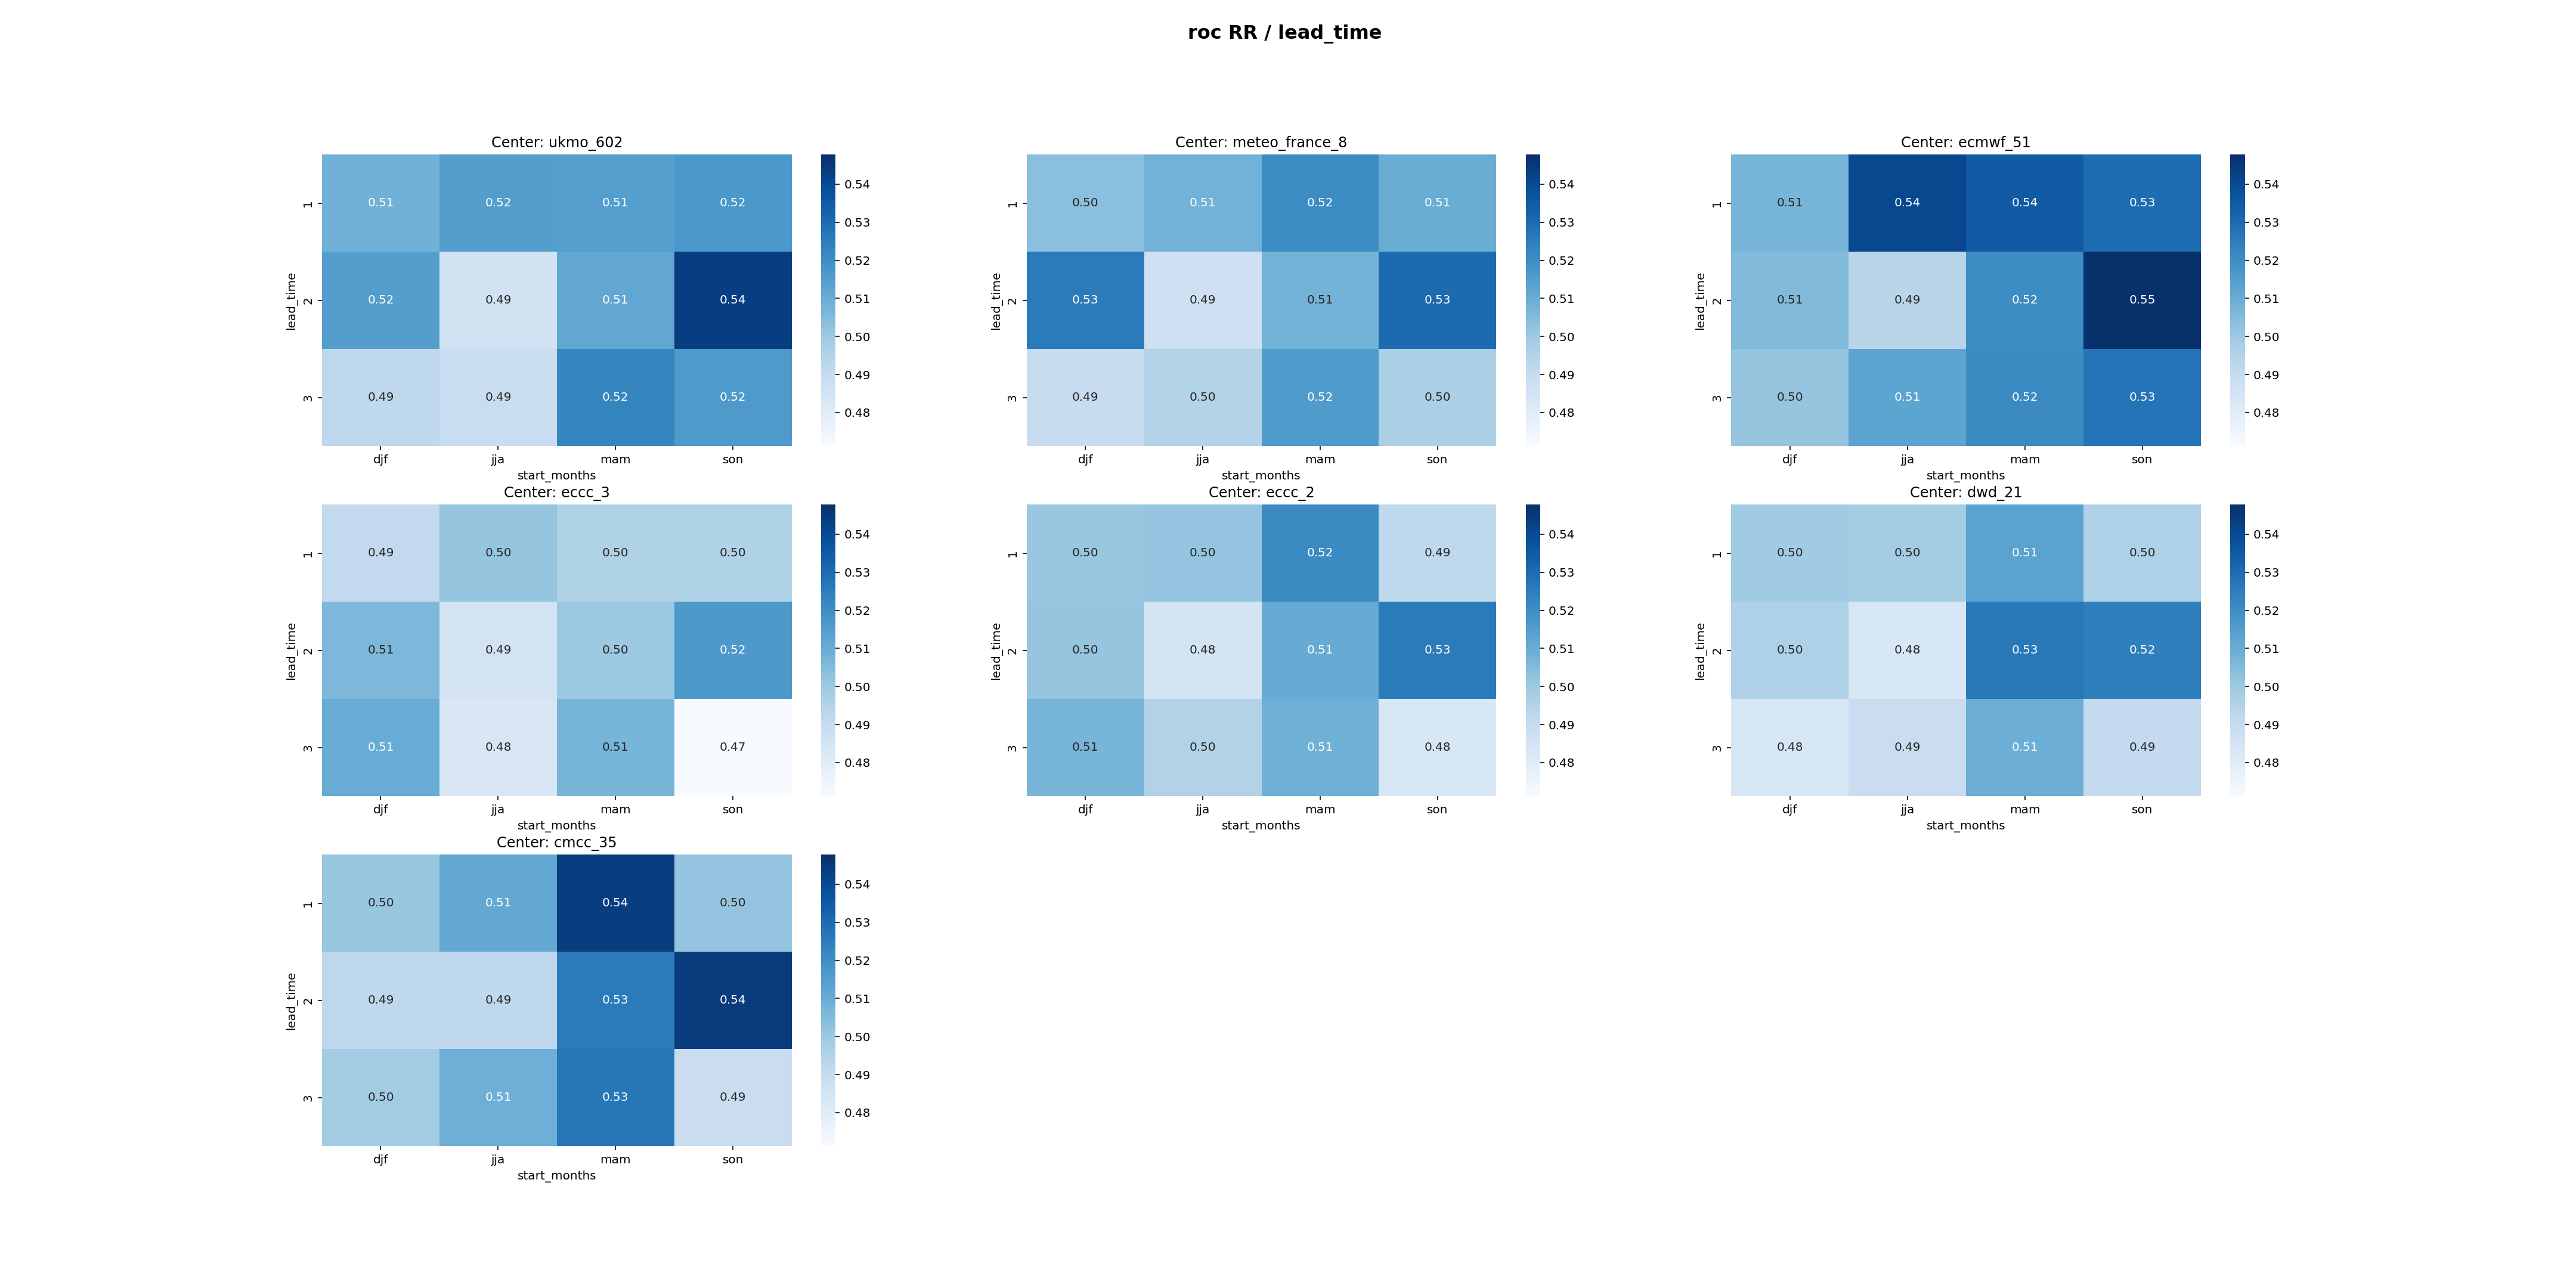
\includegraphics[scale=0.25]{plots/prob/roc/roc_RR_lead_time.png}
    \caption{The Heatmap of ROC Score for lead-times. \textbf{\textit{(1 means perfect ROC)}}}
\end{figure}

for the ROC score, all centers show similar good performance, in general the best score is observed for tha first lead-time, except for the SON season where the best performance is for the second lead-time.

\begin{figure}[H]
    \centering
    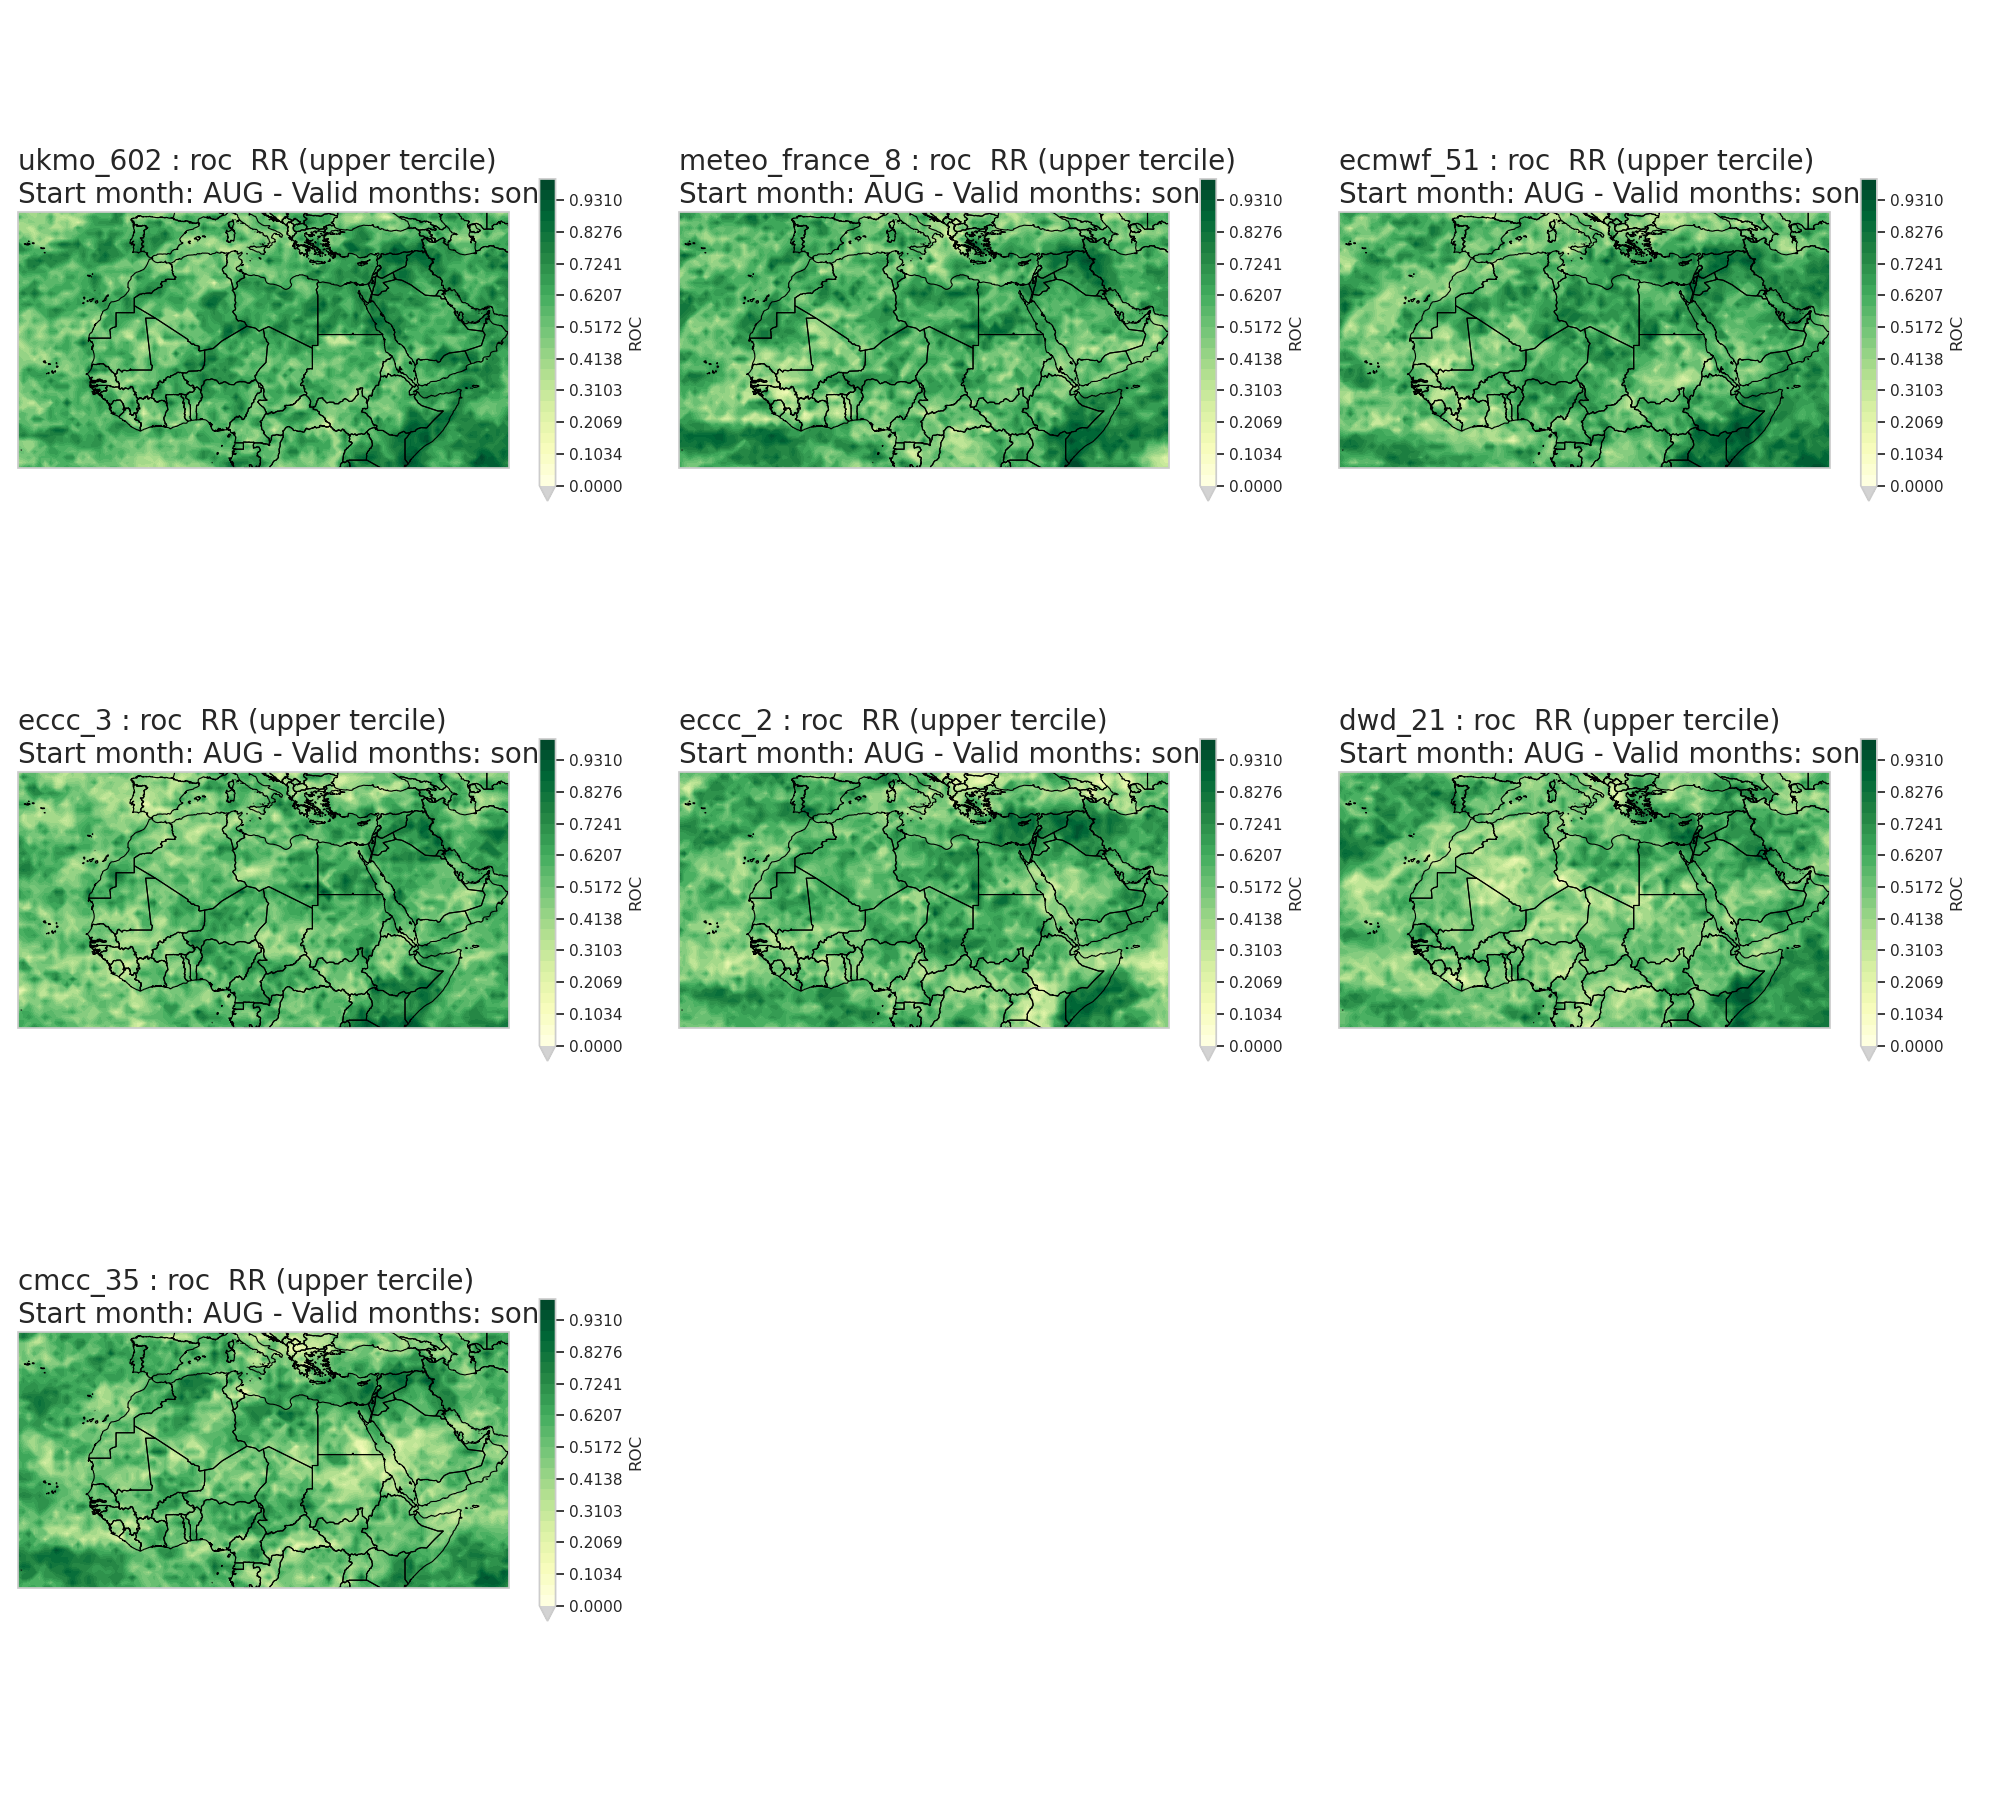
\includegraphics[scale=0.3]{plots/prob/roc/roc_son_RR_upper.png}
    \caption{The ROC Score Upper tercile SON    . \textbf{\textit{(1 means perfect ROC)}}}
\end{figure}

the spacial distribution of the roc score confirms an important result. For precipitation all centers shows better performance for the East of Africa, Irak,Syria,Jordan and Palestine. The performance in this zone is very high (score near to 1). For the rest of MENA region the performance is similar, with moderate to good score.


\subsubsection{Relative operating characteristics Skill Score}

In the figure above, the ECMWF exhibit the best performance for all terciles and periods. However, we should notice that the performance is very low for the middle tercile in all centers. For the analysis along time, the performance is so low, the best performance is in the first lead-time, except the SON which shows the best performance for the second lead-time. Above all, the \textbf{\textit{ecmwf}} shows the best performance.

\begin{figure}[H]
    \centering
    \includegraphics[scale=0.25]{plots/prob/rocss/rocss_RR_category.png}
    \caption{The ROCSS Score for each category  . \textbf{\textit{(1 means perfect ROCSS)}}}
\end{figure}


\begin{figure}[H]
    \centering
    \includegraphics[scale=0.25]{plots/prob/rocss/rocss_RR_lead_time.png}
    \caption{The average of  ROCSS Score on all categories    . \textbf{\textit{(1 means perfect ROCSS)}}}
\end{figure}



\begin{figure}[H]
    \centering
    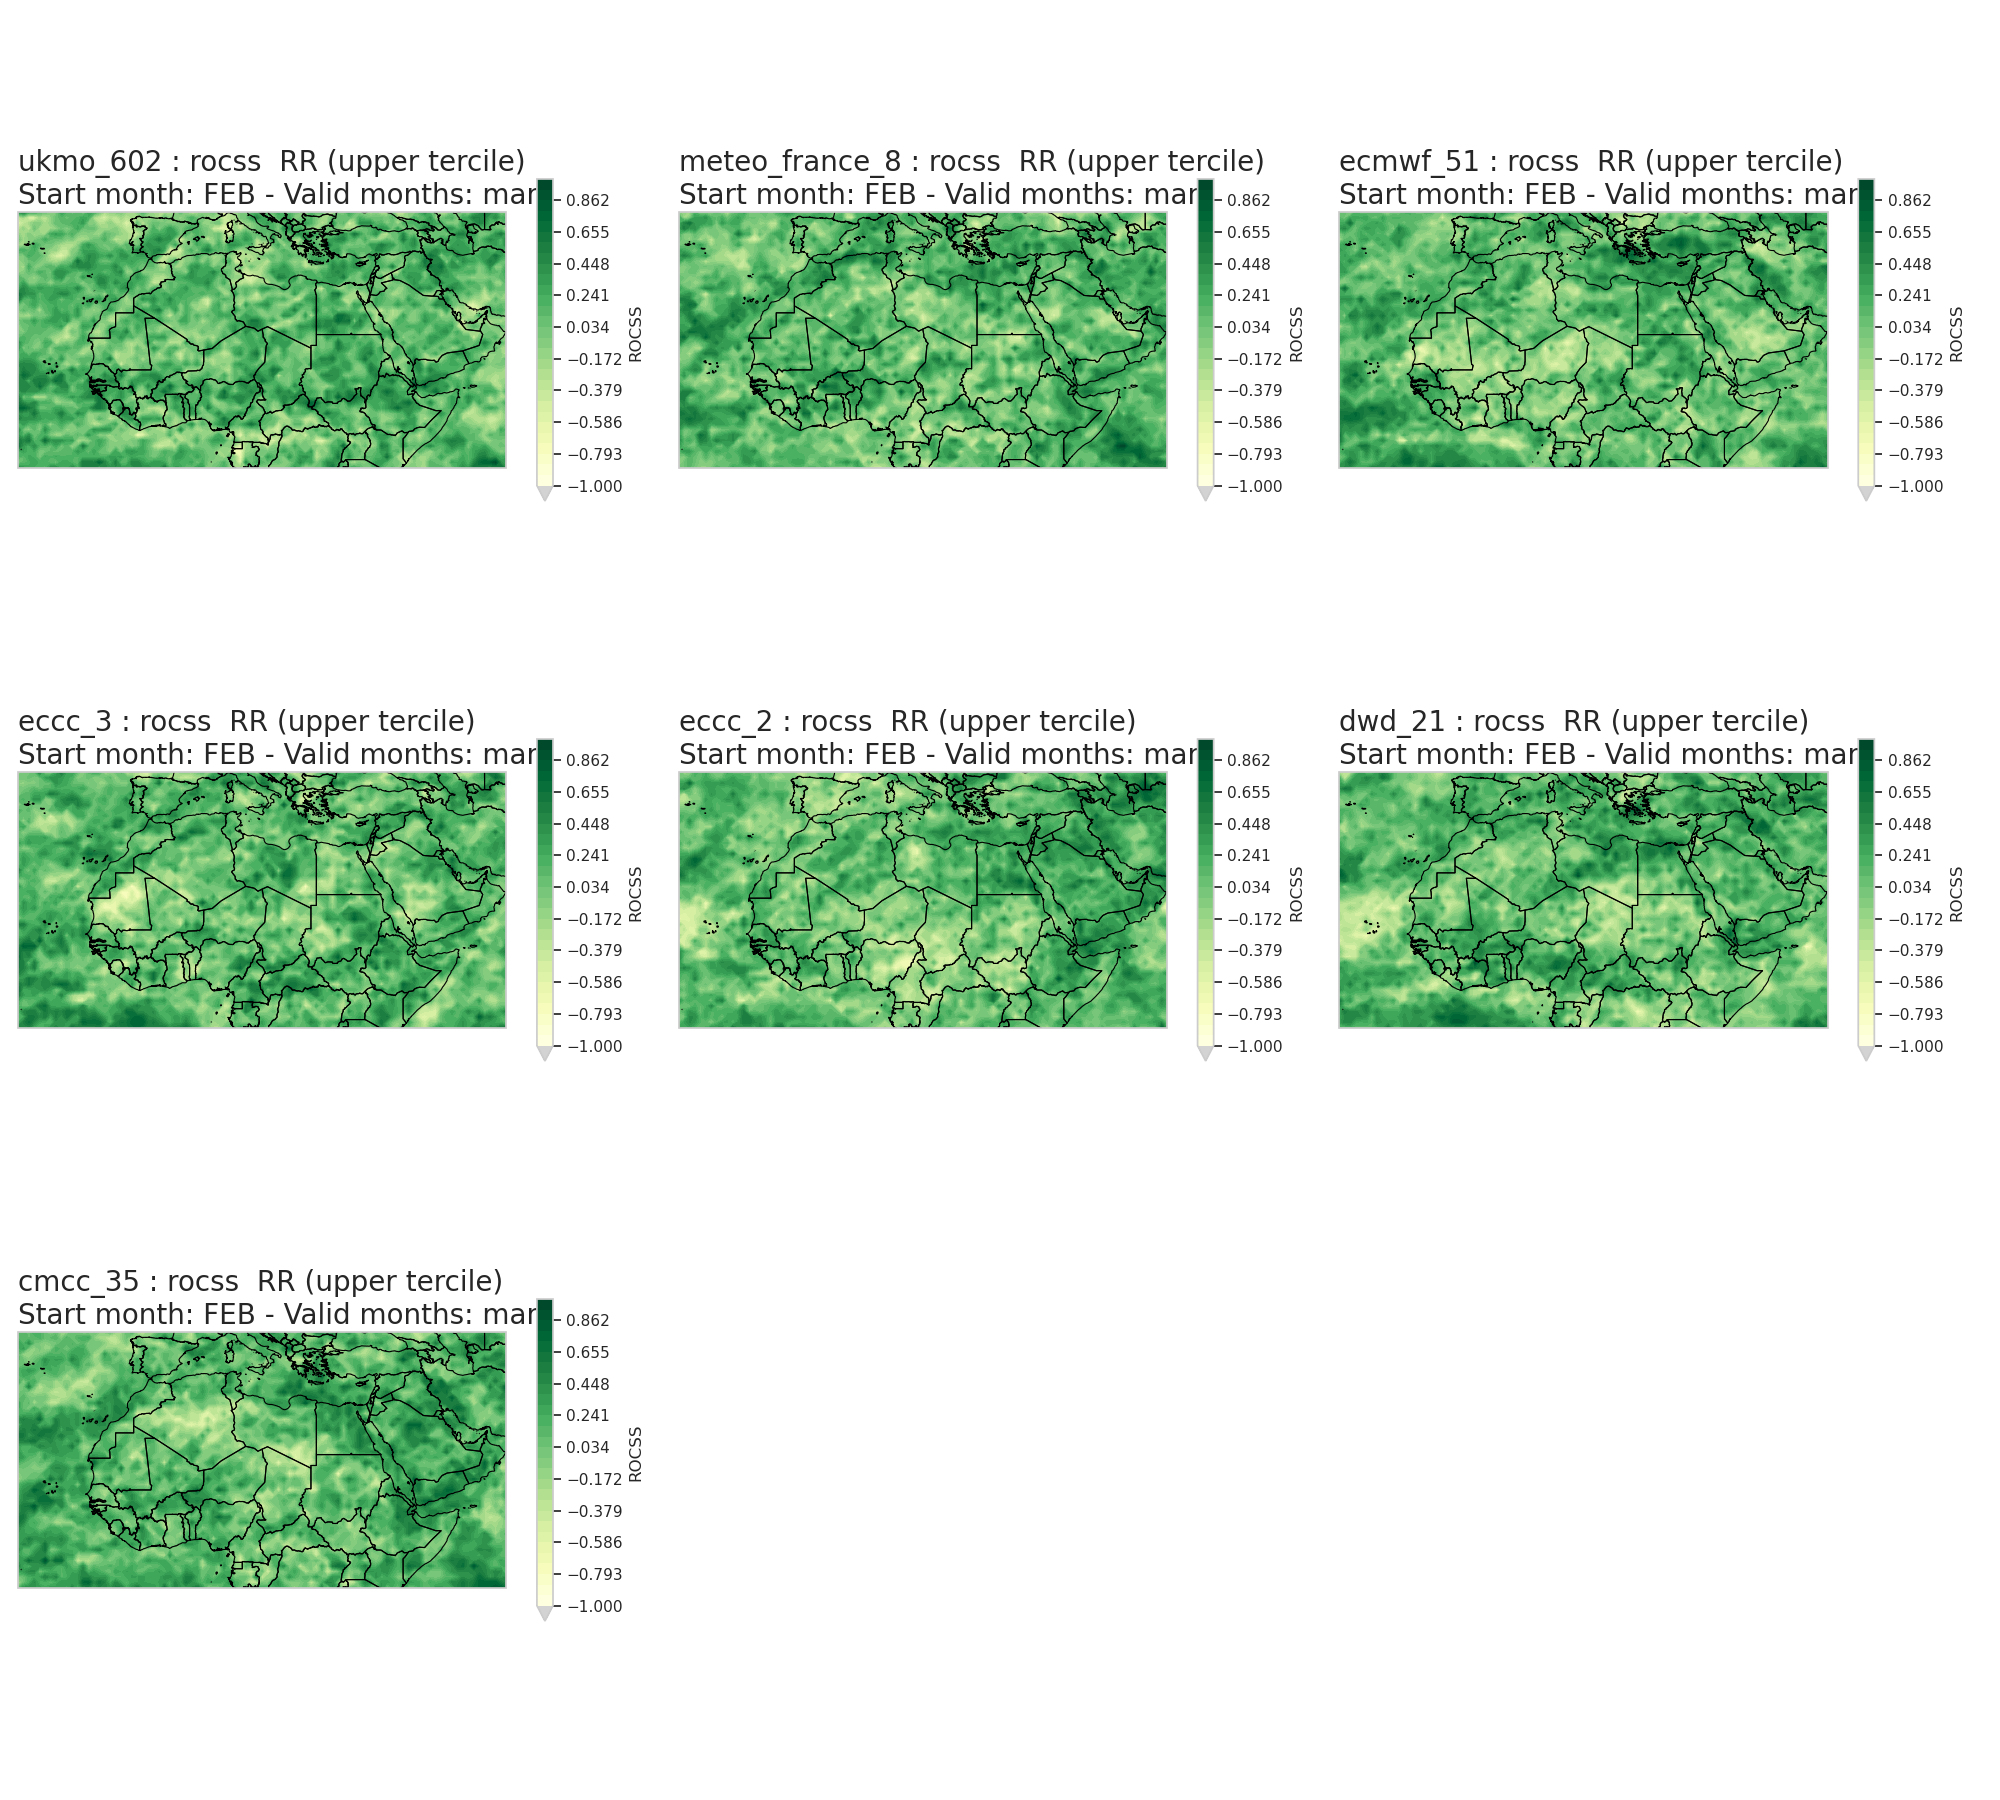
\includegraphics[scale=0.3]{plots/prob/rocss/rocss_mam_RR_upper.png}
    \caption{The ROC Skill Score Upper tercile MAM    . \textbf{\textit{(1 means perfect ROC)}}}
\end{figure}

the spacial distribution of the ROCSS, shows that all centers are consistent for this score. The spacial distribution isn't clear, there is a high spacial variability.








\subsubsection{summary}
\begin{table}[h!]
\centering
\begin{tabularx}{\textwidth}{@{}p{2.5cm}p{4cm}p{4cm}p{2.5cm}p{3cm}@{}}
\toprule
\textbf{Metric}       & \textbf{Focus}                                    & \textbf{What it Measures}                         & \textbf{Dependent on Observed Outcomes?} & \textbf{Visualization/Tools}             \\ \midrule
\textbf{Reliability}   & Probabilities match observed frequencies          & Calibration of probabilities                      & Yes                                      & Reliability diagram                      \\
\textbf{Discrimination} & Differentiating between outcomes                 & Ability to distinguish events from non-events    & Yes                                      & ROC curve, AUC                           \\
\textbf{Sharpness}     & Boldness of probabilities (away from average)     & Confidence of the forecast                        & No                                       & Histogram of forecast probabilities      \\
\textbf{Resolution}    & Informativeness and variability of forecast       & Ability to provide specific, useful info         & Yes                                      & Brier Score decomposition                \\ \bottomrule
\end{tabularx}
\caption{Key differences between reliability, discrimination, sharpness, and resolution in seasonal forecasting.}
\label{tab:forecast_metrics}
\end{table}

\newpage
\thispagestyle{empty}
\mbox{}